%%%%%%%%%%%%%%
%% Run LaTeX on this file several times to get Table of Contents,
%% cross-references, and citations.

%% w-bktmpl.tex. Current Version: Feb 16, 2012
%%%%%%%%%%%%%%%%%%%%%%%%%%%%%%%%%%%%%%%%%%%%%%%%%%%%%%%%%%%%%%%%
%
%  Template file for
%  Wiley Book Style, Design No.: SD 001B, 7x10
%  Wiley Book Style, Design No.: SD 004B, 6x9
%
%  Prepared by Amy Hendrickson, TeXnology Inc.
%  http://www.texnology.com
%%%%%%%%%%%%%%%%%%%%%%%%%%%%%%%%%%%%%%%%%%%%%%%%%%%%%%%%%%%%%%%%

%%%%%%%%%%%%%%%%%%%%%%%%%%%%%%%%%%%%%%%%%%%%%%%%%%%%%%%%%%%%%%%%
%% Class File

%% For default 7 x 10 trim size:
%\documentclass{WileySev}

%% Or, for 6 x 9 trim size
\documentclass{WileySix}

%%%%%%%%%%%%%%%%%%%%%%%%%%%%%%%%%%%%%%%%%%%%%%%%%%%%%%%%%%%%%%%%
%% Post Script Font File

% For PostScript text
% If you have font problems, you may edit the w-bookps.sty file
% to customize the font names to match those on your system.

\usepackage{w-bookps}

%%%%%%%
%% For times math: However, this package disables bold math (!)
%% \mathbf{x} will still work, but you will not have bold math
%% in section heads or chapter titles. If you don't use math
%% in those environments, mathptmx might be a good choice.

% \usepackage{mathptmx}


%%%%%%%%%%%%%%%%%%%%%%%%%%%%%%%%%%%%%%%%%%%%%%%%%%%%%%%%%%%%%%%%
%% Graphicx.sty for Including PostScript .eps files

\usepackage{graphicx}
\usepackage{enumitem}

%%%%%%%%%%%%%%%%%%%%%%%%%%%%%%%%%%%%%%%%%%%%%%%%%%%%%%%%%%%%%%%%
%% Other packages you might want to use:

% for chapter bibliography made with BibTeX
% \usepackage{chapterbib}

% for multiple indices
% \usepackage{multind}

% for answers to problems
% \usepackage{answers}




%%%%%%%%%%%%%%%%%%%%%%%%%%%%%%%%%%%%%%%%%%%%%%%%%%%%%%%%%%%%%%%%
%% Change options here if you want:
%%
%% How many levels of section head would you like numbered?
%% 0= no section numbers, 1= section, 2= subsection, 3= subsubsection
%%==>>
\setcounter{secnumdepth}{3}

%% How many levels of section head would you like to appear in the
%% Table of Contents?
%% 0= chapter titles, 1= section titles, 2= subsection titles, 
%% 3= subsubsection titles.
%%==>>
\setcounter{tocdepth}{2}

%% Cropmarks? good for final page makeup
%% \docropmarks %% turn cropmarks on

%%%%%%%%%%%%%%%%%%%%%%%%%%%%%%%%%%%%%%%%%%%%%%%%%%%%%%%%%%%%%%%%
%% DRAFT
%
% Uncomment to get double spacing between lines, current date and time
% printed at bottom of page.
% \draft
% (If you want to keep tables from becoming double spaced also uncomment
% this):
% \renewcommand{\arraystretch}{0.6}
%%%%%%%%%%%%%%%%%%%%%%%%%%%%%%

\begin{document}

%%%%%%%%%%%%%%%%%%%%%%%%%%%%%%%%%%%%%%%%%%%%%%%%%%%%%%%%%%%%%%%%
%% Title Pages
%%
%% Wiley will provide title and copyright page, but you can make
%% your own titlepages if you'd like anyway

%% Setting up title pages, type in the appropriate names here:
\booktitle{Arsitektur Komputer}
\subtitle{Mengenal Komputer Lebih Dekat}

\author{Rolly Maulana Awangga}
%\affil{Program Studi Sarjana Terapan Teknik Informatika Politeknik Pos Indonesia}
%or
%\authors{}

%% \\ will start a new line.
%% You may add \affil{} for affiliation, ie,
%\authors{Robert M. Groves\\
%\affil{Universitat de les Illes Balears}
%Floyd J. Fowler, Jr.\\
%\affil{University of New Mexico}
%}

%% Print Half Title and Title Page:
\halftitlepage
\titlepage


%%%%%%%%%%%%%%%%%%%%%%%%%%%%%%%%%%%%%%%%%%%%%%%%%%%%%%%%%%%%%%%%
%% Off Print Info

%% Add your info here:
\offprintinfo{Arsitektur Komputer, pre-release}{Rolly Maulana Awangga}

%% Can use \\ if title, and edition are too wide, ie,
%% \offprintinfo{Survey Methodology,\\ Second Edition}{Robert M. Groves}


%%%%%%%%%%%%%%%%%%%%%%%%%%%%%%%%%%%%%%%%%%%%%%%%%%%%%%%%%%%%%%%%
%% Copyright Page

\begin{copyrightpage}{2017}
Arsitektur Komputer / Rolly Maulana Awangga
\end{copyrightpage}

% Note, you must use \ to start indented lines, ie,
% 
% \begin{copyrightpage}{2004}
% Survey Methodology / Robert M. Groves . . . [et al.].
% \       p. cm.---(Wiley series in survey methodology)
% \    ``Wiley-Interscience."
% \    Includes bibliographical references and index.
% \    ISBN 0-471-48348-6 (pbk.)
% \    1. Surveys---Methodology.  2. Social 
% \  sciences---Research---Statistical methods.  I. Groves, Robert M.  II. %
% Series.\\

% HA31.2.S873 2004
% 001.4'33---dc22                                             2004044064
% \end{copyrightpage}

%%%%%%%%%%%%%%%%%%%%%%%%%%%%%%%%%%%%%%%%%%%%%%%%%%%%%%%%%%%%%%%%
%% Frontmatter >>>>>>>>>>>>>>>>

%%%%%%%%%%%%%%%%%%%%%%%%%%%%%%%%%%%%%%%%%%%%%%%%%%%%%%%%%%%%%%%%
%% Only Dedication (optional) 
%% or Contributor Page for edited books
%% before \tableofcontents

\dedication{For my family}

% ie,
%\dedication{To my parents}

%%%%%%%%%%%%%%%%%%%%%%%%%%%%%%%%%%%%%%%%%%%%%%%%%%%%%%%%%%%%%%%%
%  Contributors Page for Edited Book
%%%%%%%%%%%%%%%%%%%%%%%%%%%%%%%%%%%%%%%%%%%%%%%%%%%%%%%%%%%%%%%%

% If your book has chapters written by different authors,
% you'll need a Contributors page.

% Use \begin{contributors}...\end{contributors} and
% then enter each author with the \name{} command, followed
% by the affiliation information.

% \begin{contributors}
% \name{Masayki Abe,} Fujitsu Laboratories Ltd., Fujitsu Limited, Atsugi,
% Japan

% \name{L. A. Akers,} Center for Solid State Electronics Research, Arizona
% State University, Tempe, Arizona

% \name{G. H. Bernstein,} Department of Electrical and
% Computer Engineering, University of Notre Dame, Notre Dame, South Bend, 
% Indiana; formerly of
% Center for Solid State Electronics Research, Arizona
% State University, Tempe, Arizona 
% \end{contributors}

%%%%%%%%%%%%%%%%%%%%%%%%%%%%%%%%%%%%%%%%%%%%%%%%%%%%%%%%%%%%%%%%
\contentsinbrief %optional
\tableofcontents
% \listoffigures %optional
% \listoftables  %optional

%%%%%%%%%%%%%%%%%%%%%%%%%%%%%%%%%%%%%%%%%%%%%%%%%%%%%%%%%%%%%%%%
% Optional Foreword:

%\begin{foreword}
%text
%\end{foreword}

%%%%%%%%%%%%%%%%%%%%%%%%%%%%%%%%%%%%%%%%%%%%%%%%%%%%%%%%%%%%%%%%
% Optional Preface:

%\begin{preface}
% text
%\prefaceauthor{}
%\where{place\\
% date}
%\end{preface}

% ie,
% \begin{preface}
% This is an example preface.
% \prefaceauthor{R. K. Watts}
% \where{Durham, North Carolina\\
% September, 2004}

%%%%%%%%%%%%%%%%%%%%%%%%%%%%%%%%%%%%%%%%%%%%%%%%%%%%%%%%%%%%%%%%
% Optional Acknowledgments:

% \acknowledgments
% acknowledgment text
% \authorinitials{} % ie, I. R. S.


%%%%%%%%%%%%%%%%%%%%%%%%%%%%%%%%
%% Glossary Type of Environment:

% \begin{glossary}
% \term{<term>}{<description>}
% \end{glossary}

%%%%%%%%%%%%%%%%%%%%%%%%%%%%%%%%
% \begin{acronyms} 
% \acro{<term>}{<description>}
% \end{acronyms}

%%%%%%%%%%%%%%%%%%%%%%%%%%%%%%%%
%% In symbols environment <term> is expected to be in math mode; 
%% if not in math mode, use \term{\hbox{<term>}}

% \begin{symbols}
% \term{<math term>}{<description>}
% \term{\hbox{<non math term>}}Box used when not using a math symbol.
% \end{symbols}

%%%%%%%%%%%%%%%%%%%%%%%%%%%%%%%%
% \begin{introduction}
%\introauthor{<name>}{<affil>}
% Introduction text...
% \end{introduction}

%%%%%%%%%%%%%%%%%%%%%%%%%%%%%%%%%%%%%%%%%%%%%%%%%%%%%%%%%%%%%%%%
%% End for Front Matter, Beginning of text of book  >>>>>>>>>>>

%% Short version of title without \\ may be written in sq. brackets:

%% Optional Part :
\part[Definisi dan Software]
{Arsitektur Komputer\\ Software}


%\chapter[Windows]
%{Software\\ windows}
%% Nama Kelompok: Kelompok 1
% Kelas: D4 TI 1A
% Anggota: 1. Dezha Aidil Martha 1174025
% 		   2. Habib Abdul Rasyid 1174002
% 		   3. Muhammad Tomy Nur Maulidy 1174031
% 		   4. Nico Ekklesia Sembiring 1174095
% 		   5. Felix Setiawan Lase 1174026
% 		   6. Damara Benedikta Siolemba 1174012

\section{Sejarah Windows}
	pada awal mulanya windows muncul dengan nama QDOS (Quick and Dirty Operating System) yang ditulis oleh Paterson dari Seatle Computer pada tahun 1980.
Kemudian pada tahun 1981 Bill gates dari microsoft membeli licensi QDOS tersebut dan mengganti namanya menjadi MS-DOS seiring perkembangan dari tahun ke tahun namanya berubah menjadi Windows seperti yang kita ketahui sekarang ini.
\subsection{kelebihan windows}
	1.	sistem operasi yang user friendly
	2.	dukungan hardware yang lengkap
	3.	mendukung sistem berkas dengan format FAT,FAT16,FAT32, NTFS dan ISO
\subsubsection{Kekurangan}
	1.	rentan terkena virus
	2.	harga licensi yang cukup tinggi
	3.	tidak ada efek 3D dan resolusi gambar yang rendah.


\section{Macam - macam Windows dan penjelasannya}

% Windows 3.1 
\subsection{Sejarah Windows 3.1}
\ref{Windows31}
	Windows 3.1 memiliki sistem operasi 16 bit, diproduksi oleh microsoft untur client, pertama kali dikeluarkan pada 6 April 1992 sebagai versi lanjutan dari Windows 3.0 \cite{brodsky1996just}
	\subsubsection{Karakteristik Windows 3.1}
		1.Dirilis pada tanggal 6 April 1992
		2.Mendukung software multimedia
		3.Menggunakan mkernel hibrida
		4.Diperkenalkan sistem berkas NTFS
	\subsubsection{Sistem keamanan Windows 3.1}
		1.Keamanan masih kurang bagus
		2.Tidak ada pembatasan user untuk menggunakan OS
		3.Rentan terhadap virus
	\subsubsection{Kelebihan Windows 3.1}
		1.Memudahkan komunikasi antar anggota workgroup
		2.Dukungan driver yang lebih banyak
		3.Lebih mudah mengakses file dan aplikasi di komputer lain
		4.Administrasi sistem jaringan relatif lebih mudah
	\subsubsection{Kekurangan}
		1.Virus gampang menyerang OS
		2.Sering terjadi maintenence, tetapi masih belum mengatasi virus
		3.Sistem nya kurang stabil

\begin{figure}[ht]
\centerline{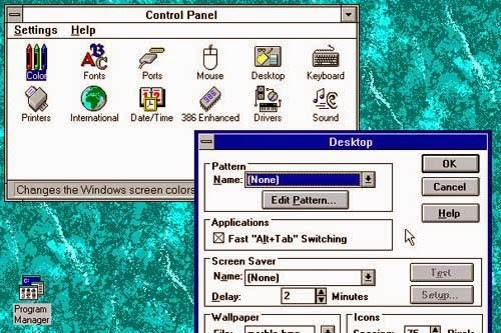
\includegraphics[width=1\textwidth]{figures/Windows31.JPG}}
\caption{tampilan desktop di windows 3.1}
\label{Windows31}
\end{figure}

% Windows 95
\section{windows 95}
\ref{desktop95}
	Windows 95 merukapan sistem operasi hubruda 16-bit/32-biit dan 
	diproduksi oleh microsoft, windows ini di perkenalkan kepada 
	publik pada tanggal 14 agustus 1995. Windows 95 ini adalah produk 
	pertama windows dengan kernel monolotic yg berjalan  -/+  60 tanpa dos 
	dan di dalamnya sudah berisi microsoft office 1995. \cite{petzold1996programming} 
	\subsection{Lima versi windows 95}
		1.windows 95
		2.windows 95 A
		3.windows 95 B
		4.windows 95 B USB
		5.windows 95 C


\begin{figure}[ht]
\centerline{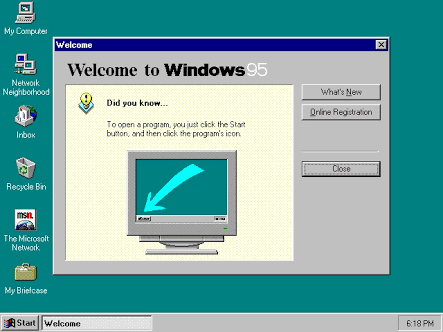
\includegraphics[width=1\textwidth]{figures/desktop95.PNG}}
\caption{tampilan desktop di windows 95.}
\label{desktop95}
\end{figure}

% Windows 98
\section{windows98}
		\ref{Desktopwindows98}
	windows 98 adalah pengembangan dari windows 95 dimana windows 98 diluncurkan agar lebih stabil daripada versi sebelumnya, windows versi 98 ini adalah versi pertama yang dibuat secara spesifik untuk konsumen. pada windows 98 ini memiliki fitur menarik yang disebut \"Deskbar\" fitur ini bisa mengunduh bilah alat desktop(deskbar) dari situs-situs favorit mereka.
	Dalam sebuah artikel dari davis menyebutkan bahwa revisi dari windows 98 adalah pemasangan dan perubahan antarmuka hingga komponen built-in, perangkat tambahan dan multimedia baru dan bagian referensi teknis yang jauh kebih luas. \cite{Davis:1998:W9B:551711}
	\subsection{fitur tambahan dari windows 98}
			Pada windows 98 ini mencakup banyak driver dan dukungan berkas system FAT32.
		Dalam sebuah artikel dari mcfedries menyebutkan bahwa windows 98 memiliki fitur windows terbaru, anda dapat menemukan Internet Explorer 4.0 dan Active Desktop; mengatur Outlook Express untuk surat internet dan surat CompuServer; Instalasi,konfigurasi, dan kostumisasi windows 98 termasuk dua-boot; membuka potensi multimedia windows 98 \cite{mcfedries1998windows}

		\begin{figure}[ht]
		\centerline{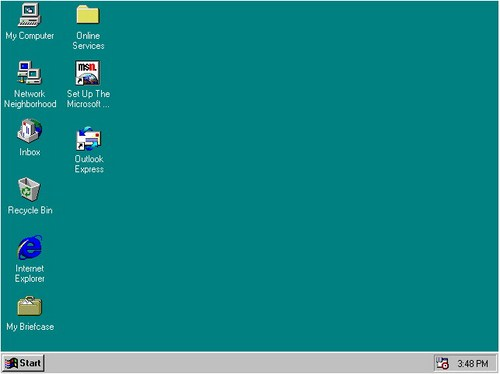
\includegraphics[wiedth=1\textwidth]{figures/Desktopwindows98.JPG}}
		\caption{tampilan desktop windows 98}
		\label{Desktopwindows98}
		\end{figure}

% Windows 2000
\section{windows2000}
	Windows 2000 diluncurkan oleh perusahaan multinasional Microsoft Corporation pada tanggal 17 Februari 2000 di Washington, Amerika Serikat. 
	Dalam sebuah buku yang ditulis oleh Solomon disebutkan bahwa Windows 2000 merupakan flatform dari sistem operasi generasi lanjutan dari windows seri NT4.0 dan menyediakan fitur-fitur lebih tinggi,ekstensi aritmatika yang lebih kuat dan akurat, memiliki instruksi khusus untuk multimedia, serta mendapat dukungan memori yang besar dari chip Intel 64-bit dengan fitur multiprocessing yang luas \cite{solomon2000inside}
	\subsection{tujuan perancangan windows 2000}
		Pada awal pembuatannya, Windows 2000 dirancang untuk memenuhi kebutuhan akan bisnis yang dilakukan melalui dunia maya seperti e-commerce, data dari suatu tempat, proses transaksi online, dan aplikasi yang memiliki performa tinggi.
	\subsection{fokus pengembangan windows 2000}
		Fokus pengembangan Windows 2000 terdapat pada bidang keandalan sistem dan diharapkan sistem operasi baru yang diluncurkan pada saat itu lebih dapat diandalkan dari sistem operasi yang lain.
		Dalam artikel yang ditulis oleh Murphy, tidak adanya standar industri yang ditujukan untuk mengkarakterisasi keandalan sistem menuntut Microsoft agar menambahkan fungsionalitas kerja kedalam sistem operasinya agar lebih dapat diandalkan dan mengurangi persepsi pelanggan mengenai terjadinya bug dan masalah yang akan terjadi dalam penggunaan fungsi dan fitur-fitur baru dasi sistem operasi yang baru ini. Sehingga pelangga akan merasa nyaman dalam menggunakan sistem operasi yang baru ini \cite{murphy2000windows} 

% Windows 2003 server
\section{windows 2003 server}
\ref{windows2003server}
	windows 2003 adalah pembaruan dari windows 2000 server yang menggabungkan kompatibilitas dan fitur-fitur lainnya dari windows XP, alasan windows 2003 ini menggunakan metode kompatibilitas agar aplikasi lama dapat bekerja dengan stabiLitas yang besar, semua itu dibuat kompatibel dengan jaringan yang berbasis windows NT 4.0 . pada windows 2003 ini menawarkan berbagai fitur keamanan baru, seperti \"Manage Your Wizard\".
	dalam sebuah artikel yang ditulis oleh Litch Field menyebutkan bahwa windows 2003 dirancang agar aman diluar kontak. Sebagian dari keamanan diadopsi oleh microsoft untuk versi windows terbaru dengan tujuan mengurangi resiko yang ditimbulan oleh kerentangan buffer offerflow \cite{litchfield2003defeating}
	\subsection{edisi windows server 2003}
		windows server 2003 menggunakan kernel windows NT versi 5.2 
		windows server 2003 tersedia dalam lima buah edisi:
		1.windows server 2003 standart edition
 		2.windows server enterprise edition (32bit dan 64bit)
		3.windows server datacenter edition
		4.windows server small business server
		5.windows strorage server 2003


\begin{figure}[ht]
\centerline{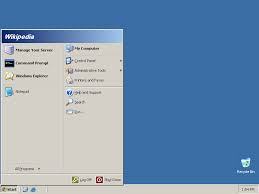
\includegraphics[width=1\textwidth]{figures/windows2003server.JPG}}
\caption{tampilan desktop di windows 2003 server}
\label{windows2003server}
\end{figure}
% Windows XP
	\section{Windows XP}
		Windows XP dirilis setelah Windows 2000 dan Windows Me (millenium edition), Windows XP sebelumnya dikenal dengan sebutan sandi Whistler. Dan pertama kali dipublikasikan tanggal 25oktober 2001. Windows XP adalah kependekan dari Windows Experience yang artinys pengalaman. Windows XP mempunyai daya tarik tersendiri karena Windows XP merupakan Windows pertama yang dibangun diatas kernel dan arsitektur Windows NT.\cite{pogue2002windows}\ref{windowsxp}
		\subsection{jenis Windows XP}
			1.Windows XP Professional
			2.Windows XP Home Edition
			3.Windows XP Media Center Edition
			4.Windows XP Tablet PC Edition
			5.Windows XP Starter Edition
			6.Windows XP Professional X64 Edition
			7.Windows XP Professional 64-Bit Edition for Itanium
		\subsection{fiture dan peningkatan}
			Windows XP menggabungkan home line dengan corporate line nya sehingga menjadi sistem terpadu yang sangat baik. Windows XP memiliki kestabilan dan efisieni yang telah melebihi Windows 98, Windows ME, dan Windows 2000 professional, hal ini disebabkan Windows XP memiliki software untuk menghindari yang disebut dengan \"neraka DLL\" atau \"DLL HELL\".
			\subsubsection{Stabilitas}
				Jika suatu program rusak, program itu tidak akan mengganggu memori yang digunakan program lain. Inilah tindakan tindakan microsoft untuk membuat PC stabil:
		 			a. Perlindungan file sistem
		 			b. Manajemen lebih berhati hati
		 			c. Sistem otomatis update
			\subsubsection{Perubahan tampilan}
				Windows XP telihat lebih bagus dengan taskbar dan Windows berwarna biru terang. juga ikon memiliki tampilan gelap 3D
			\subsubsection{Gmabar, Musik, dan Film}
				Windows XP mendapatkan penghargaan karena telah memasukan kamera digital ke dalam PC.
			\subsubsection{Dukungan terhadap sistem domain Active Directory} 
				Active Directory merupakan suatu sistem yang dapat diatur dari satu tempat saja, yaitu dari sistem yang menjalankan sistem itu sendiri. Fitur ini dapat meneyderhanakan 	proses autentikasi di perusahaan perusahaan besar.
			\subsubsection{Peningkatan pengaturan kontrol akses}
				Windows XP ditujukan untuk penggunaan korporasi,sehingga telah dilengkapi dengan pengaturan kontrol akses. Fitur ini digunakan untuk membatasi akses yang tidak memiliki izin akses terhadap objek tertentu.
			\subsubsaction{Mendukung sistem bekas terenskripsi}
				Fiture ini digunakan untuk melindungi data data penting sehingga tidak dapat dibuka orang lain, kecuali dengan membuka kodenya.

\begin{figure}[ht]
\centerline{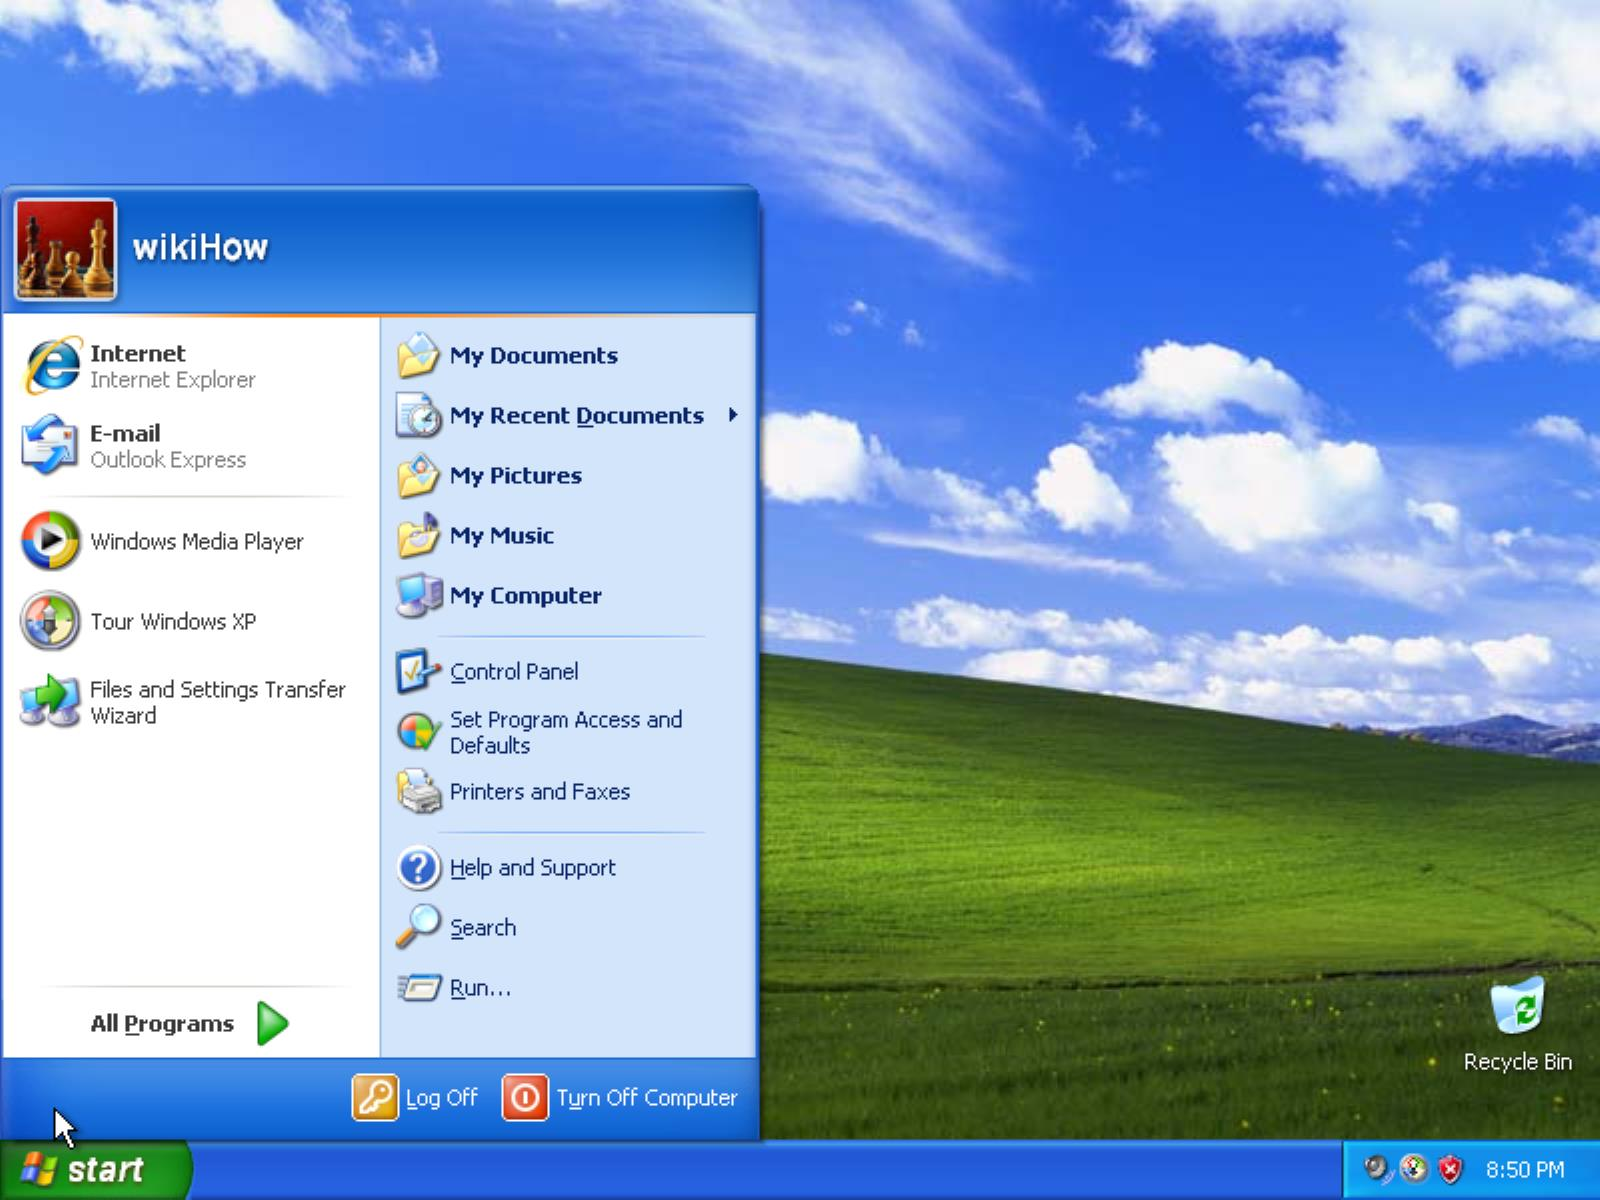
\includegraphics[width=1\textwidth]{figures/windowsxp.JPG}}
\caption{tampilan desktop di windows XP}
\label{windowsxp}
\end{figure}
% Windows Vista
	\section{Sejarah Windows Vista}
\ref{vista1}
		Windows Vista adalah sistem operasi berbasis dari Microsoft pada PC, Windows Vista dirilis pada tanggal 22 Juli 2005, Windows Vista ini lebih dikenal dengan Longhorn
	\subsection{Kelebihan dan Kekurangan Windows Vista}  \cite{russinovich2009windows}
		\subsubsection{Kelebihan:}
			1. Kualitas warna yang lebih tinggi, sehingga GUI (Grhapic User Interface) lebih bagus
			2. Bisa membaca RAM up to 16 GB
			3. Mendukung direct X 10
			4. Lebih cepat menjalankan program
			5. Banyak fitur baru yang tidak ada dalam versi sebelumnya
			6. Pencarian file lebih mudah 
		\subsubsection{Kekurangan:}
			1. Terdapat beberapa aplikasi yang belum support
			2. Terlalu banyak varian seri
	\subsection{Spesifikasi Hardware}
		\subsubsection{Minimum}
			Processor 800 Mhz(Pentium III atau Athlon)
			RAM 512 Mb
			Hard disk 40 Gb
			Graphic card bebas
		\subsubsection{Medium}
			Processor 2Ghz(Pentium 4 2,6 Ghz, Athlon XP 2800+ dll)
			RAM 1024 Mb
			Hard disk Sata 80 Gb
			Graphic card Direct x 9.0 (128 - 256 MB)
		\subsubsection{High}
			Processor 3 Ghz atau lebih, Processor Dual Core
			RAM 2048 Mb DDR II
			Hard disk Sata 120 Gb
			Graphic card Pixel Shader 2/3. (>256 MB)


\begin{figure}[ht]
\centerline{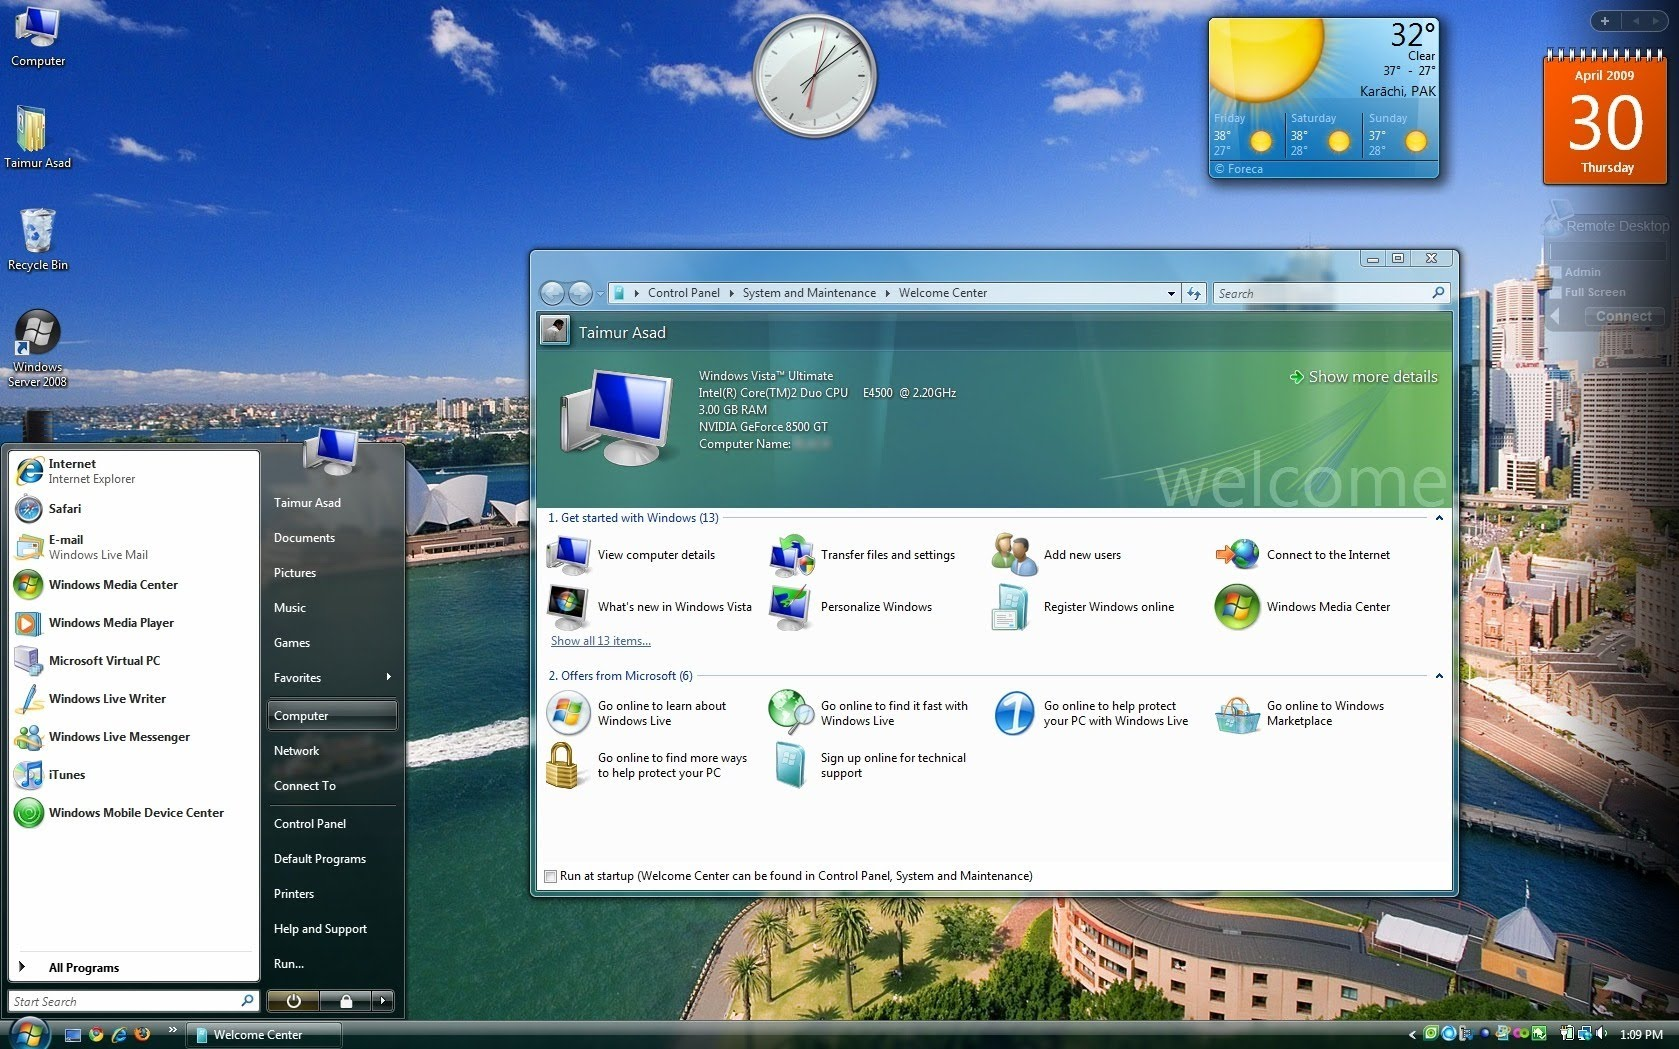
\includegraphics[width=1\textwidth]{figures/vista1.JPG}}
\caption{tampilan desktop di windows vista}
\label{vista1}
\end{figure}


% Windows 7
	\section{windows 7}
\ref{desktop7}
		Ada fitur fitur baru di windows 7 yang memberikan tantangan untuk memori
		dan juga menawarkan informasii yang dapat dipulihkan dan di ambil dari
		gambar,file,dan makalah. Fitur baru di windows 7 ini di kembangkan 
		metode analisis memori sesuai fitur masing masing. Metode ini
		berlandasan pada struktur data windows yangbernama dengan kernel
		processor. Proses yang berjalan pada windows ini ada 2 yaitu windows 7 
		7 dan 64-bit dan 32-bit windows 7
		\subsection{pendahuluan}
			Memori komputer sangat lah berguna sebagai sumber daya juga menawarkan
			Semua sistem operasi sepenuhnya dijalankan COROM, dan hampir semua
			semua informasi berhaga ada di memori komputer.
		\subsection{windows 7 edisi}
			1.windows 7 starter.
			2.windows 7 prefessional.
			3.windows 7 home basic.
			4.windows 7 enterprise.
			5.windows 7 ultimate.
			6.windows 7 home premium.
		\subsection{analisi windows 7 dan memori}
			\subsubsection{Gambaran dari windows 7}
				Ada pun perbadingan dengan widows 2000 dan windows xp, fitur windows 7 
				dijelaskan sebangai berikut. Strktur KPCR terletak di virtual OxFFDFFOOO
				di windows 7 KPCR dan KPCRB berada tidak terletak di alamat ini karna
				alamat struktur KPCR tidak dapat di temukan oleh lokasi stirng biner 
				00fdfff0fldff dalam gambar memo.(2) masing-masing objek karel adalah 
				prefxed oleh struktur objek header di windows 2000, dalam object header
				struktur windows 7, type variabel adalah bukan dengan variabel 
				Typelndex.(3)log peristiwa jendela telah berubah di windows 7. Fornat 
				yang bary untuk event log dan perpanjangan baru adalah \“EVTX\” 
				dan terletak di \“C: \Windows\System32\winevvt\Logs\”
		\subsubsection{alamat terjemahan}
			Karena alamat di memori umumnya di simpan sebagai alamat virtual,dan 
			alamat fisik digunakan untuk analasisi memori maka pentung untuk 
			menerjemahkan alamat virtual tersebut ke alamat fisik dengan 
			mempelajari terjemahan alamat prosesor intel. Proses terjemahan :  
			(1) Akuisisi struktur KPCR, variabel CurrentPrcb berikut nya ke 
			variable Self. Nilai variable diri diteruskan ke variavle currentPrcb 
			subsection(Registri)
			Registri windows adalah terdiri dari sejumlah fles biner yang berbeda 
			disebut juga dengan gatal-gatal pada disk. Sarang fles adalah unit 
			alokasi yang disebut blok. Blok utama dari sarang adalah blok dasar.

\cite{zhang2010exploratory} 

\begin{figure}[ht]
\centerline{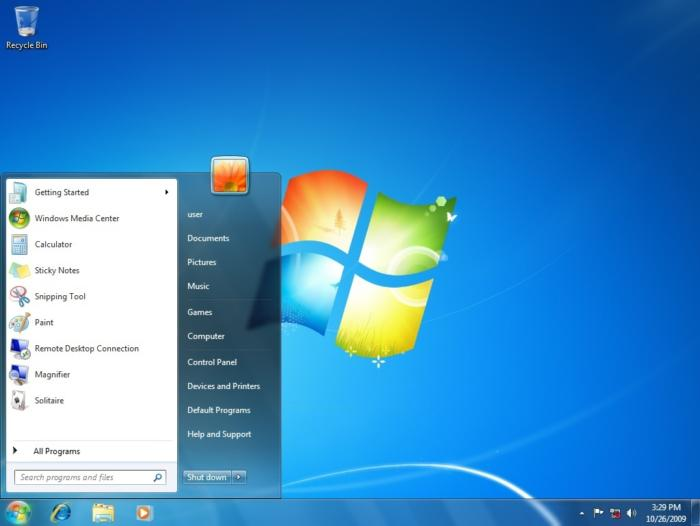
\includegraphics[width=1\textwidth]{figures/desktop7.JPG}}
\caption{tampilan desktop di windows 7}
\label{desktop7}
\end{figure}

% Windows server 2008
	\section{Windows Server 2008}
\ref{windowsserver2008}
	Windows Server 2008 merupakan sebuah sistem operasi yang powerful untuk PC server dan jaringan komputer. Windows Server 2008 diterbitkan sekitar 9 tahun yang lalu, tepatnya bulan februari tahun 2008.\cite{wahyono2009practice}
	\subsection{Sejarah dan Perkembangan}
		Sistem operasi Windows NT masih ada kaitannya dengan perkembangan Windows Server. Tahun 2007 Windows Server yang dikenal dengan nama \" Windows Server Codenamed Longhorn\" dikembangkan oleh microsoft. Longhorn diciptakan untuk menggantikan Windows Server 2003. Sesuai dengan keputusan Bill Gates tanggal 15 mei 2007 Windows Server Longhorn berubah menjadi Windows Server 2008.
	\subsection{Spesifikasi Sistem}
		\subsubsection{Prosesor}
		Minimal 1 GHz (X86 Processor) atau 1.4 GHz (x64 Processor)
		\subsubsection{Memori}
		Minimal yang dibutuhkan adalah 512 MB RAM. Maksimum untuk 32-Bit adalah 4 GB(standar) atau 64 GB(Enterpise dan Datacenter). Untuk yang 64-Bit Maksimumnya adalah 8 GB (Foundation), 32 GB (Standar), dan 2 TB (Enterpise, Datacenter, dan Itanium)
		\subsubsection{Hardisk}
		Minimum untuk 32-Bit adalah 20 GB dan untuk 64-Bit adalah 32 GB.
		\subsubsection{Display}
		Minimal Super VGA (800 x 600). Tetapi untuk pengalaman yang lebih baik menggunakan resolusi yang lebih tinggi.
	\subsection{Fitur penting}
	Windows Server 2008 mempunyai arsitektur dan fungsional lebih maju dibandingkan para pendahulunya. Dan juga memiliki kelibihin instalasi yang lebih mudah, diagnosis kesalahan, dan keamanan yang tangguh.

\begin{figure}[ht]
\centerline{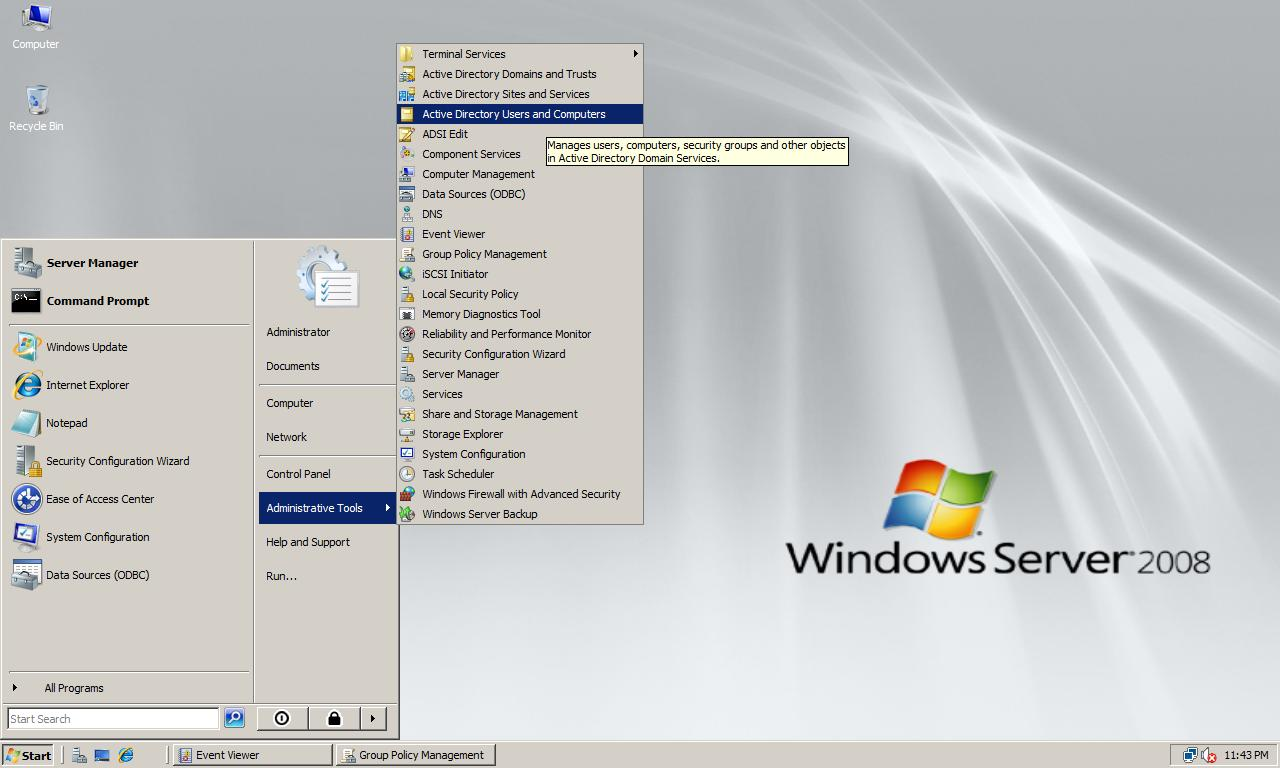
\includegraphics[width=1\textwidth]{figures/windowsserver2008.JPG}}
\caption{tampilan desktop di windows server 2008}
\label{windowsserver2008}
\end{figure}
% Windows 8
	\section{windows 8}
		\ref{tampilanwindows8} windows 8 diluncurkan oleh microsoft pada tahun 2012. dengan dirilisnya windows 8 ini mengubah format file hibernasi, memecah semua alat analisis yang ada.
		Dalam artikel yang ditulis oleh sylve mengemukakan bahwa pada saat itu matthieu suiche mempelajari format file hibernasi windows modern, pada bulan mei 2016 suiche mengumumkan versi beta Hibr2Bin yang mendukung file hibernasi windows 8. Hibr2Bin adalah alat yang mengubah file hibernasi windows menjadi gambar memori mentah sehingga bisa dianalisis dengan alat analisis memori yang secara native tidak mendukung penguraidan file hibernasi. Hibr2Bin diperbarui dan rilis secara terbuka pada akhir september 2016. \cite{sylve2017modern}
		\subsection{Fitur tambahan pada windows 8}
			Seperti yang di kutip pada artikel wahyu asri, windows 8 memiliki fitur tambahan yang memiliki kelebihan sebagai berikut :
			1. Optimalisasi untuk layar sentuh
			2. mendukung chip ARM
			3. toko aplikasi windows store
			4. mendukung NFC (Near Field Communication)
			5. waktu boot yang singkat
			6. Internet Explore 10
			7. Security lebih baik
			8. windows 8 tidak membutuhkan upgrade PC \cite{wahyu8review}

\begin{figure}[ht]
\centerline{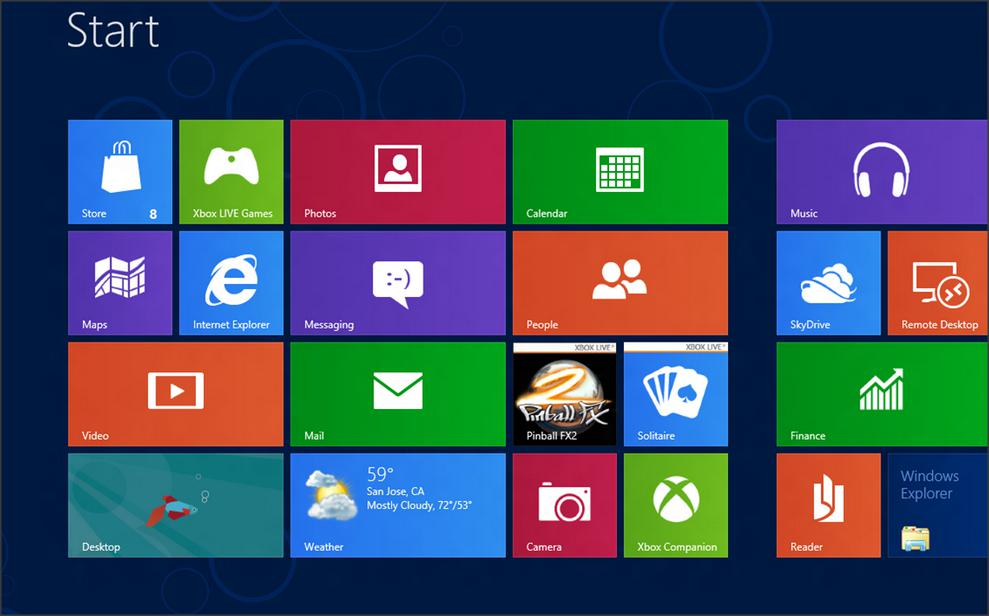
\includegraphics[width=1\textwidth]{figures/tampilanwindows8.JPG}}
\caption{tampilan desktop di windows 8.}
\label{tampilanwindows8}
\end{figure}


% Windows 2012 server
	\section{windows 2012 server}
		\ref{windows12} windows 2012 server merupakan sistem operasi penyempuraan dari windows sebelumnya yaitu windows 2008 R2. Windows 2012 ini merupakan versi server windows 8, pada windows 2012 ini, 
		menawarkan berbagai fitur-fitur baru dan juga peningkatan-peningkatan pada windows server. Windows ini resmi diperkenalkan pada november 2012. Tidak seperti windows 2008 R2 windows 
		2012 server ini tidak memiliki dukungan komputer yang berbasis itanium dan pada windows 2012 server ini banyak menekankan penggunaan cloud pribadi, sehingga pengguna dapat 
		mengaplikasikan dengan mudah. pada windows 2012 ini juga membantu memudahkan pengguna untuk menginstal mesin virtualnya secara efisien. disamping itu windows 2012 ini memiliki beberapa
		fitur untuk memperbaiki windows 2008 R2. dengan adanya semua fitur yang ada pada windows 2012 tersebut pengguna akan dapat mempelajari segala sesuatu mulai dari instalisasi, 
		keamanan, konfigurasi otomasi, pemantauan dan lain sebagainya yang dimuat dalam format resep praktis\cite{carvalho2012windows}
		\subsection{edisi windows server 2012}
			1.windows server 2012 foundation
			2.windows server 2012 essantiasis
			3.windows server 2012 standard
			4.windows server 2012 datacenter
			5.windows multipoint server 2012

\begin{figure}[ht]
\centerline{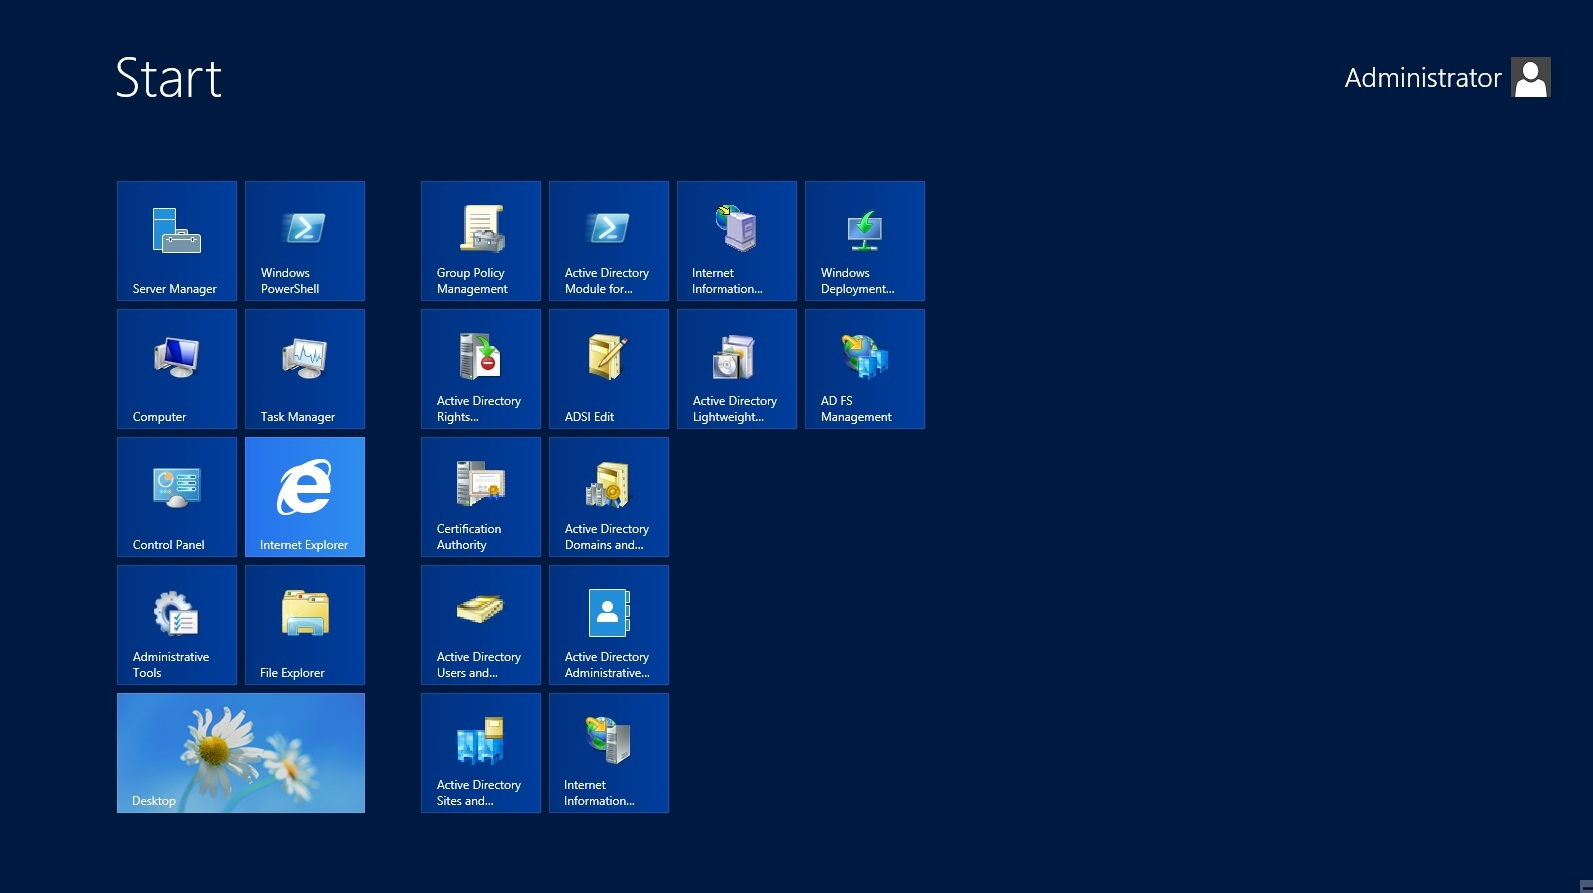
\includegraphics[width=1\textwidth]{figures/windows12.JPG}}
\caption{tampilan desktop di windows server 2012}
\label{windows12}
\end{figure}

	
% Windows 10
	\section{windows10}
		Windows 10 merupakan salah satu sistem operasi yang dirilis oleh perusahaan multinasional Microsoft Corporation pada tanggal 29 juli 2015. windows 10 dikenal sebagai suatu sistem 
		operasi yang selalu menerima pembaharuan terhadap fitur fitur yaang ada didalamnya. Pada awal peluncurannya, Microsoft Corporation mengadakan sebuah kampanye periklanan yang 
		mengenai perilisan windows 10 yang memiliki tema \"Upgrade Your World\". Dalam iklan tersebut, perusahaan ini menggunakan tagline \"Cara Yang Lebih Manusiawi Untuk Diakses\" berikut gambar dari windows 10 \ref{tampilanwindows10}
		\subsection{keunggulan dan fitur fitur windows 10}
			Dalam sebuah buku yang ditulis oleh JJ. Foster menyebutkan sistem operasi versi terbaru dari Microsoft ini mampu membangun keselarasan pengalaman dan fungsionalitas pengguna 
			dalam perbedaan kelas perangkat \cite{foster2001data} 
			Pada fitur windows 10 terdapat Windows Store yang berfungsi sebagai wadah untuk mendownload aplikasi. gambar ditampilkan sebagai berikut\ref{Store}, Groove Music sebagai 
			aplikasi pemutar musik. gambar ditampilkan sebagai berikut\ref{Groove}, dan Films dan Tv sebagai aplikasi pemutar video dan film. Gambar ditampilkan sebagai berikut\ref{Films_Tv}. 
			Tidak hanya itu, Windows 10 juga menyedikan fitur Xbox yang memungkinkan para pengguna untuk menjelajah perpustakaan permainan. Gambar ditampilkan sebagai berikut\ref{Xbox}
		\subsection{fitur yang dihapus}
			Akan tetapi, ada juga fitur yang tidak dilanjutkan pengembangan bahkan dihapus saat diupgrade dari versi sebelumnyl.a. Fitur tersebut adalah:
			-Windows Media Center
			-Aplikasi makanan dan minuman
			-Aplikasi kesehatan
			-dan aplikasi travel/perjalanan.


\begin{figure}[ht]
\centerline{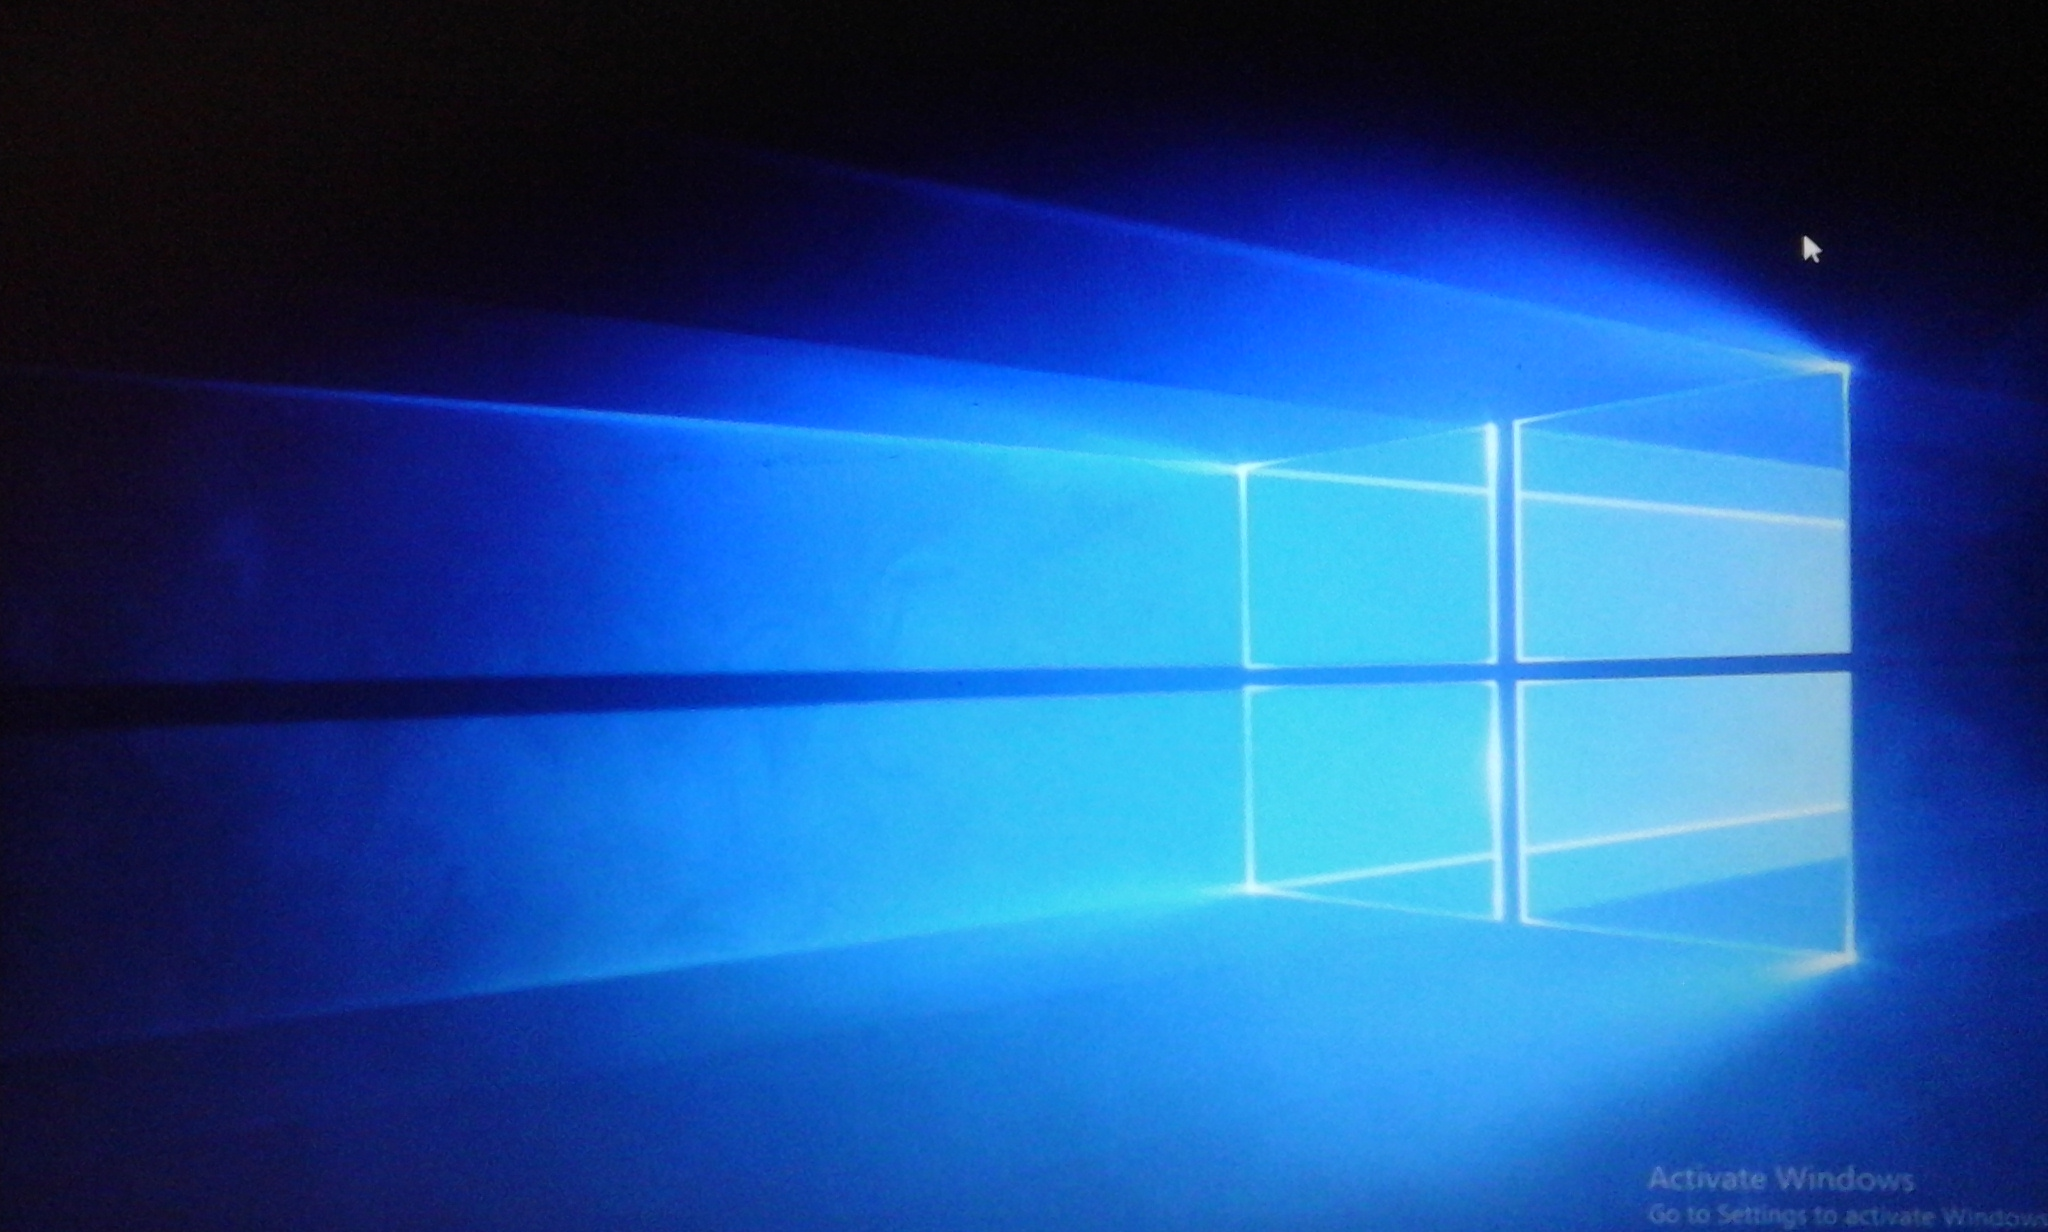
\includegraphics[width=1\textwidth]{figures/tampilanwindows10.JPG}}
\caption{tampilan desktop di windows 10.}
\label{tampilanwindows10}
\end{figure}

\chapter[Linux]
{Software\\ linux}
% Nama Kelompok : Linux
% Kelas : D4 TI 1A
% 1. Kadek Diva Krishna Murti (1174006)
% 2. Duvan Silalahi (1174011)
% 3. Oniwaldus (1174005)
% 4. Choirul Anam (1174004)
% 5. Sri Rahayu (1174015)
% 6. Ilham Habibi (1174028)



\begin{figure}[ht]
\centerline{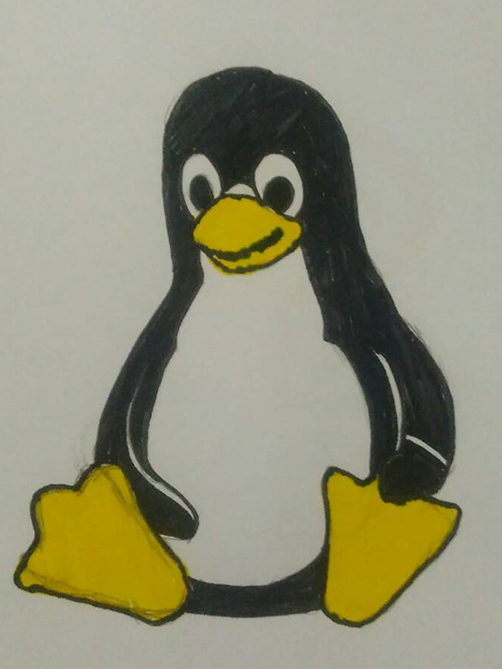
\includegraphics[width=0.5\textwidth]{figures/linux.jpg}}
\caption{Logo Linux.}
\label{Linux}
\end{figure}

Menurut Wahana Komputer dalam bukunya yang berjudul Mari Mengenal Linux menyebutkan bahwa Linux merupakan sebuah sistem operasi yang mirip dengan UNIX, dan merupakan implementasi independen dari sistem operasi POSIX, dengan ekstensi SYSV dan BSD sistem operasi UNIX, yang berjalan di mesin keluarga Intel 80386DX, atau yang lebih baru. Pada perkembangan berikutnya, Linux dapat berjalan di beberapa mesin lainnya seperti Sun Sparc, Mac, PowerPC, DEC Alpha, dan PPC mk86.\cite{komputer2005mari}

Linux adalah sistem operasi yang diedarkan secara gratis di bawah lisensi GNU General Public License (GPL), yang berarti source code Linux tersedia. Dengan begitu program tersebut dapat diubah, diadaptasi, maupun dikembangkan lebih lanjut oleh siapapun.

\section{Sejarah} 

Menurut Wahana Komputer dalam bukunya yang berjudul Mari Mengenal Linux menyebutkan bahwa dahulu Linux adalah proyek hobi yang dikerjakan oleh seorang mahasiswa Finlandia yang bernama Linus Torvalds. Dalam mengerjakan proyek hobinya tersebut, Linus Torvalds memperoleh inspirasi dari Minix, yaitu suatu sistem UNIX kecil yang dikembangkan oleh Andy Tanenbaum. Linux versi 0.01 dikerjakan sekitar bulan Agustus 1991. Kemudian pada tanggal 5 Oktober 1991 Linus Torvalds mengumumkan versi resmi dari Linux, yaitu 0.02. Versi ini hanya dapat menjalankan Bash (GNU Bourne Again Shell) dan gcc (GNU C Compiler). Meskipun Linux bukan merupakan sistem Unix resmi, namun Linux memiliki dasar warisan, budaya, arsitektur dan pengalaman sistem operasi Unix, sebuah sistem operasi yang sudah berjalan selama 28 tahun lebih. \cite{komputer2005mari}

\subsection{Pengenalan}

Menurut artikel Dasar-Dasar Linux menyebutkan bahwa Linus Torvalds membuat Kernel Linux, yaitu sebuah core Linux, di atas Minix dengan menggunakan bahasa C. Linux memiliki lisensi GNU, sebuah lisensi yang dikeluarkan untuk memungkinkan seseorang mendistribusikan, mengembangkan, dan memodifikasi source code suatu program secara gratis dan bebas. Pembuatan Linux di lakukan secara gotong royong oleh banyak programmer yang kebanyakan C/C++ Programmer di seluruh dunia via internet. Logo Linux adalah seekor penguin seperti gambar\ref{Linux}. Karena pada saat pengembangan Linux, Torvalds pernah di patuk oleh Penguin di sebuah kebun binatang yang menyebabkan dirinya demam dan dia bercita-cita agar orang lain dapat \"demam\" Linux. Nama Linux sendiri di adaptasi dari nama nya Linus. Saat ini, Linux memiliki beberapa Desktop Environment yang berbasis Grafis yaitu, KDE (K Desktop Environment) dan GNOME (GNU Network Object Model Environment). \cite{sofwan2003dasar}

\subsection{Aplikasi Yang Terdapat di Linux}

Menurut Wahana Komputer dalam bukunya yang berjudul Mari Mengenal Linux menyebutkan bahwa karena kernel Linux dikembangkan dengan usaha yang independent, banyak aplikasi yang tersedia, sebagai contoh, C Compiler menggunakan gcc dari Free Software Foundation GNU’s Project. Compiler ini banyak dipergunakan  pada lingkungan Hewlett-Packard dan Sun. Sekarang, banyak aplikasi Linux yang dapat dipergunakan untuk keperluan perkantoran seperti untuk spreadsheet, word processor, database dan Star Office yang merupakan program editor grafis yang memiliki tampilan dan fungsi layaknya Microsoft Office. Selain itu di Linux juga sudah tersedia versi Corel dan aplikasi seperti Matlab yang pada Linux dikenal sebagai Scilab. \cite{komputer2005mari}

Sekarang Linux merupakan sistem UNIX yang bisa digunakan untuk jaringan (networking), pengembangan software, bahkan untuk kebutuhan sehari-hari. Linux merupakan alternatif sistem operasi yang bisa didapatkan secara gratis jika dibandingkan dengan sistem operasi komersial lainnya dan dengan kemampuan yang setara atau bahkan lebih.


\section{Distribusi Linux}

Berikut ini beberapa distribusi (distro) Linux yang banyak peminatnya di Indonesia.

\begin{enumerate}

\item \textbf{Debian Linux}

\begin{figure}[ht]
\centerline{
\includegraphics[width=0.4\textwidth]{figures/debian.jpg}}
\caption{Logo Debian Linux.}
\label{Debian}
\end{figure}

Menurut Wahana Komputer dalam bukunya yang berjudul Mari Mengenal Linux menyebutkan bahwa Debian merupakan distribusi dari Linux yang kurang terkenal, namun banyak penggunanya dari kalangan teknis. Mereka puas karena kestabilannya. Selain itu, format paket programnya yang menggunakan DEB dianggap lebih stabil daripada RPM menurut kalangan teknis.
Versi terakhir dari Debian adalah versi 2.1, yang dirilis pada tahun 1999. Dibandingkan dengan distribusi lainnya, Debian termasuk yang jarang dalam meng-update programnya. Debian juga sudah menggunakan metode autodetect untuk penggunaan peripheral pada komputer. \cite{komputer2005mari} Debian Linux memiliki logo seperti gambar \ref{Debian}.

Jika Anda ingin tahu lebih lanjut mengenai Debian Linux ataupun men-download programnya secara langsung, Anda bisa mengunjungi situsnya di http://www.debian.org

\textbf{\item RedHat Linux}


\begin{figure}[ht]
\centerline{
\includegraphics[width=0.4\textwidth]{figures/redhat.jpg}}
\caption{Logo RedHat Linux.}
\label{RedHat}
\end{figure}

Menurut Wahana Komputer dalam bukunya yang berjudul Mari Mengenal Linux menyebutkan bahwa  Redhat merupakan distribusi Linux yang paling popular di Indonesia dan Amerika yang dirancang khusus untuk server. RedHat di akui sebagai server tercepat dibandingkan dengan distribusi Linux lainnya untuk server. Selain dapat diguanakan sebagai server tercepat, RedHat juga dapat dipakai sebagai klien maupun digunakan sebagai desktop rumah tangga alias PC standlone. Saat ini Redhat sudah beredar dengan versi 6.2, menggunakan Standard Desktop Gnome.

Kelebihan lain dari RedHat adalah kemudahan dalam hal instalasinya. Ini merupakan revolusioner Linux. Ketika distribusi linux lainnya membuat penggunanya awalnya menjadi putus asa pada saat prosedur instalasinya, RedHat hadir dengan prosedur instalasi yang termudah pada masanya.
Hal revolusioner lainnya adalah RedHat membuat format paket program RPM menjadi standar baku file biner pada Linux, yang kemudian digunakan oleh distribusi lainnya seperti SuSE, Mandrake dan Caldera. \cite{komputer2005mari} Redhat Linux memiliki logo seperti gambar \ref{RedHat}.

Jika Anda ingin tahu lebih lanjut mengenai RedHat Linux ataupun men-download programnya secara langsung, Anda bisa mengunjungi situsnya di http://www.redhat.com

\textbf{\item Mandrake Linux}


\begin{figure}[ht]
\centerline{
\includegraphics[width=0.4\textwidth]{figures/mandrake.jpg}}
\caption{Logo Mandrake Linux.}
\label{Mandrake}
\end{figure}

Menurut Wahana Komputer dalam bukunya yang berjudul Mari Mengenal Linux menyebutkan bahwa Mandrake adalah saudara muda dari RedHat, karena keduanya dibuat oleh satu distribusi. Bila RedHat direkomendikasikan sebagai server, maka Mandrake direkomendasikan oleh pembuat distro RedHat sebagai klien yang handal, namun diutamakan yang menggunakan prosesor Pentium. Meskipun demikian, tidak menutup kemungkinan penggunaan Mandrake sebagai server yang handal juga.

Tujuan diciptakannya Mandrake pada awalnya adalah untuk mempermudah penggunanya dalam melakukan instalasi dan penggunaan Linux. Sebelum diluncurkannya Corel Linux, Mandrake merupakan salah satu distribusi Linux yang paling populer. Jika RedHat keluar dengan desktop manager menggunakan Gnome, maka Mandrake keluar dengan desktop manager KDE buatan SuSE Jerman. Saat ini Mandrake sudah keluar dengan versi 7.1. \cite{komputer2005mari} Mandrake Linux memiliki logo seperti gambar \ref{Mandrake}.

Jika Anda ingin tahu lebih lanjut mengenai Mandrake Linux ataupun men-download programnya secara langsung, Anda bisa mengunjungi situsnya di http://www.linux-mandrake.com

\textbf{\item Caldera Open Linux}


\begin{figure}[ht]
\centerline{
\includegraphics[width=0.4\textwidth]{figures/caldera.jpg}}
\caption{Logo Caldera Open Linux.}
\label{Caldera}
\end{figure}

Menurut Wahana Komputer dalam bukunya yang berjudul Mari Mengenal Linux menyebutkan bahwa Caldera merupakan merupakan distribusi Linux yang dirancang untuk mempermudah pemakainya dalam pengoperasiannya. Caldera sendiri dirancang sebagai distribusi Linux yang keselurahannya dalam bentuk grafis. Sejak mulai instalasi hingga setting hardware, semuanya dalam bentuk grafis. Yang mengagumkan adalah pada saat melakukan instalasi Caldera, Anda akan disuguhi game tetris untuk mengisi waktu, sembari menunggu transfer program. Selain itu Caldera merupakan distribusi Linux pertama yang menggunakan auto-detect hardware (seperti plug dan  play pada Mac). \cite{komputer2005mari} Caldera Linux memiliki logo seperti gambar \ref{Caldera}.

Jika Anda ingin tahu lebih lanjut mengenai Caldera Open Linux ataupun men-download programnya secara langsung, Anda bisa mengunjungi situsnya di http://www.caldera-system.com

\textbf{\item Slackware Linux}


\begin{figure}[ht]
\centerline{
\includegraphics[width=0.4\textwidth]{figures/slackware.jpg}}
\caption{Logo Slackware Linux.}
\label{Slackware}
\end{figure}

Menurut Wahana Komputer dalam bukunya yang berjudul Mari Mengenal Linux menyebutkan bahwa Slackware dibuat oleh Patrick Volkerding, Slackware merupakan distribusi Linux yang pertama, dengan tampilan yang sederhana tapi penggunaannya manual tidak seperti produk Linux yang lain. Biasanya Slackware digunakan oleh pengguna Linux yang sudah pro atau bisa juga yang ingin menjadi pengguna Linux yang pro. Slackware awalnya turunan dari Softlanding Linux System dan merupakan yang paling populer dari distribusi Linux asli. Versi Slackware Linux yang pertama tersedia di publik adalah versi 1.0 yang rilis pada 16 juli 1993. Slackware Linux mengacu pada prinsip KISS (Keep It Simple Stupid). \cite{ komputer2005mari}. Slackware Linux memiliki logo seperti gambar \ref{Slackware}.

Jika Anda ingin tahu lebih lanjut mengenai Slackware Linux ataupun men-download programnya secara langsung, Anda bisa mengunjungi situsnya di http://www.slackware.com

\textbf{\item Suse Linux}


\begin{figure}[ht]
\centerline{
\includegraphics[width=0.4\textwidth]{figures/suse.jpg}}
\caption{Logo Suse Linux.}
\label{Suse}
\end{figure}

Menurut Wahana Komputer dalam bukunya yang berjudul Mari Mengenal Linux menyebutkan bahwa Suse Linux merupakan distribusi Linux yang sistemnya dioperasikan di atas kernel. Suse Linux merupakan produk Linux yang sangat populer di Negara Eropa. Dilengkapi dengan KDE dan central setting YaST (Yet Another Settup Tools) yang digunakan sebagai sistem operasi untuk deskop dan server. Suse bermula pada tahun 1990-an yang didirikan oleh perusahaan Novell yang dimana Linux terdiri dari 50 keping disket dan dapat di unduh atau diambil lewat internet. Ada 2 macam jenis Suse Linux yaitu, Suse Linux Enterprise dan Open Suse. Suse Linux Enterprise terdiri dari 2 paket yaitu, Suse Linux Enterprise Server dan Suse Linux Enterprise Deskop. Open Suse merupakan sebuah proyek masyarakat yang disponsori oleh Novell dan dirancang untuk pengguna rumah. \cite{komputer2005mari} Suse Linux memiliki logo seperti gambar \ref{Suse}.

Jika Anda ingin tahu lebih lanjut mengenai Suse Linux ataupun men-download programnya secara langsung, Anda bisa mengunjungi situsnya di http://www.suse.com

\textbf{\item Corel Linux}


\begin{figure}[ht]
\centerline{
\includegraphics[width=0.4\textwidth]{figures/corel.jpg}}
\caption{Logo Corel Linux.}
\label{Corel}
\end{figure}

Menurut Wahana Komputer dalam bukunya yang berjudul Mari Mengenal Linux menyebutkan bahwa Corel Linux dibuat oleh distribusi Linux yaitu Debian. Corel Linux mendukung operasi sistem open source dibawah naungan GNU. Harganya juga sangat terjangkau dan dapat langsung di instal dengan sistem operasi lain dan juga bisa tanpa sistem operasi lain. Corel Linux juga bisa dinstal pada partisi dan file sistem Windows yang menjadikan corel linux seolah-olah adalah program aplikasi Windows. Corel Linux dirancang sebagai End-User. Pada Corel Linux semuanya serba grafis, dimulai saat instalasi sampai pada boot sistem. Pada Corel Linux kita tidak akan menjumpai baris teks seperti pada Linux yang lain, atau bahkan seperti pada Windows yang masih kelihatan baris teks. Semua sistem Corel Linux ini sangat sederhana sampai pada setting jaringannya lebih sederhana daripada Windows. \cite{komputer2005mari} Corel Linux memiliki logo seperti gambar \ref{Corel}.

Jika Anda ingin tahu lebih lanjut mengenai Corel Linux ataupun men-download programnya secara langsung, Anda bisa mengunjungi situsnya di http://www.linux.corel.com

\textbf{ \item Turbo Linux}


\begin{figure}[ht]
\centerline{
\includegraphics[width=0.4\textwidth]{figures/turbo.jpg}}
\caption{Logo Turbo Linux.}
\label{Turbo}
\end{figure}

Menurut Wahana Komputer dalam bukunya yang berjudul Mari Mengenal Linux menyebutkan bahwa Turbo Linux sangat populer dan terkenal di Asia. Turbo Linux menduduki posisi pertama pada Linux pilihan. Turbo Linux diciptakan dari berbagai program-program under Linux atau UNIX. Turbo Linux mendesain produknya dengan menggabungkan beberapa kelebihan dari open source dan dari perangkat lunak komersial. Turbo Linux menyertakan Cross Platform Management Software dalam produk-produk work station server dan clustering yang memungkinkan kemudahan dalam memanage networks dan sistem. Ada beberapa fitur Turbo Linux yaitu, Kernel 2.4.5, Glibc 2.2.3, Gcc 2.95.3, Xfree86 4.1.10, Rpm 4.0.2, Kde 2.1.2, Gnome 1.4. \cite{komputer2005mari} Turbo Linux memiliki logo seperti gambar \ref{Turbo}.

Jika Anda ingin tahu lebih lanjut mengenai Turbo Linux ataupun men-download programnya secara langsung, Anda bisa mengunjungi situsnya di http://www.turbo-linux.com



\end{enumerate}

\section{Kelebihan Linux}

Berikut ini beberapa kelebihan dari penggunaan Sistem Operasi Linux, di antaranya adalah:

\begin{itemize}

\item Merupakan salah satu sistem operasi yang bersifat open source, yang berarti penggunanya dapat melihat maupun mengubah source codenya tanpa terkena sanksi.

\item Merupakan salah satu sistem operasi yang freeware di bawah lisensi GNU, yang berarti penggunanya tidak harus mengeluarkan biaya untuk memiliki sistem operasi ini.

\item Tidak memerlukan spesifikasi hardware yang tinggi untuk menjalankan sistem operasi ini.

\item Linux kebal  terhadap virus karena Linux mendukung adanya file permissions (ijin file), yang dapat mencegah perubahan atau penghapusan file tanpa ijin dari pemiliknya.

\item Lebih dari satu orang dapat menggunakan program yang sama atau berbeda dari satu mesin yang sama, pada saat bersamaan, di terminal yang sama atau berbeda.

\item Dalam satu komputer, pengguna dapat melakukan login dengan nama user yang sama atau berbeda lebih dari satu kali, tanpa perlu menutup sesi sebelumnya.

\item Mengeksekusi suatu program dan mengakses data dapat dilakukan secara bersama-sama tanpa harus khawatir terjadi hang atau stack.

\item Dalam penggunaannya Linux sangat stabil sehingga bisa mengcopy, mengedit, menghapus satu file atau data secara bersamaan pada saat data atau file tersebut dieksekusi.

\item Jumlah login user atau operator yang dimiliki tidak terbatas sehingga user bisa mencapai 254 klien secara bersamaan dan dilengkapi dengan password.

\item Linux dapat digunakan sebagai Web Server atau sebagai FTP Server.

\item Linux mendukung fasilitas GUI (Graphic User Interface).

\end{itemize}

\section{Kelemahan Linux}

Berikut ini beberapa kelemahan dari penggunaan Sistem Operasi Linux, di antaranya adalah:

\begin{itemize}

\item Cara penggunaanya sangat berbeda sekali dengan sistem operasi lainnya seperti Windows sehingga perlu waktu dan tenaga ekstra untuk mempelajari penggunaanya. Apalagi bagi yang baru belajar komputer akan mengalami kesulitan dalam penggunaannya.

\item Banyak aplikasi-aplikasi yang belum mendukung penggunaanya dalam Linux.

\item Tidak dapat mendukung beberapa hardware-hardware tertentu.

\item Sedikit penggunanya, hal ini menyebabkan sedikit juga orang-orang yang dapat di jadikan ajang bertanya sesama pengguna Linux.

\end{itemize}


\chapter[Macintosh]
{Software\\ mac}
% Nama Kelompok : Macintosh
% Kelas : D4 TI 1A
% Anggota : 
% 1. Harun   	1174027
% 2. Fahmi   	1174021
% 3. Kukuh		1174016
% 4. Izzah		1174013
% 5. Rizal		1174014
% 6. Lawimner	1174030




Artikel tentang sejarah Mac OS dari masa ke masa

\section{penjelasan singkat}
Sebelum kita mengetahui lebih dalam lagi tentang MAC OS sebaiknya kita mengenal penciptanya terlebih dahulu
pada zaman dahulu kala hiduplah seorang anak yang bernama \"Steve Jobs\" yang lahir di kota San Fransisco California 
pada tanggal 24 Februari 1955. ia adalah seoarang yatim piatu yang di adopsi oleh Paul dan Clara Jobs.
Berikut perjalanan hidup dan karir Steve Jobs hingga embusan nafas terakhir : 

1955 : di tahun 1955 beliau lahir pada tanggal 24 Februari

1972 : beliau mmelanjutkan pendidikan di perkuliahan tepatnya di Reed College, Portland, Oregon. Tapi ia di drop out setelah semester pertama masuk kuliah

1974 : ia bekerja untuk pembuatan video game Atari dan mengikuti ia juga berkesempatan mengikuti pertemuan Homebrew Computer Club dengan Steve Wozniak, seorang teman sekolahnya yang lebih tua beberapa tahun dengannya. dan Ini merupakan sejenis seminar atau juga bisa di sebut dengan pertemuan yang membahas tema-tema komputer

1975 : Jobs dan Woz kembali menghadiri acara di Homebrew Computer Club Meetings. 

1976 : Komputer Apple tercipta pada April Mob yang jatuh pada tanggal 1 April, tak lama sejak itu jobs dan wozniak membuat sebuah komputer sirkuit baru di garasi Silicon Valley. Pendiri ketiga Apple, Ron Wayne, meninggalkan kerja sama ini, karena setelah hanya dua minggu bekerja. Komputer Apple I dijual pada musim panas seharga US\$ 666,66 atau sekitar Rp.8.658.000 per unit nya

1977 : Apple bergabung dengan beberapa pihak perusahaan untuk membuat kerja sama join venture. Dari situ terciptalah Apple II, komputer pribadi pertama dengan menggunakan grafis berwarna. Pendapatan perusahaan mencapai US\$ 1 juta.

1979 : selanjutnya Jobs mengunjungi Xerox Palo Alto Research Center (PARC). Dari sini ia mendapatkan sebuah ide untuk membuat sebuah komputer dengan graphical user interface yang sangat luas yaitu dapat memfasilitasi tampilan dengan pilihan pada layar berbentuk simbol-simbol 

1980 : Apple kembali mencatatkan sahamnya di bursa saham. Perusahaan mendapatkan dana sebesar US\$ 110 juta. Ini merupakan initial public offering (IPO) terbesar di tahun itu

1982 : adapun Pendapatan per tahun nya perusahaan Apple meningkat hingga mencapai US\$ 1 miliar

1983 : Komputer Apple II dengan menu ikon di layar atau mereka menamakan komputer ini The Lisa diluncurkan ke pasaran dan membuat kehebohan. beliau membujuk John Sculley untuk meninggalkan pekerjaannya di Pepsico Inc. untuk menjadi CEO di perusaan Apple

1984 : untuk meningkatkan daya jual Icon Macintosh di iklankan secara komersial selama acara Super Bowl.dan Macintosh mulai dijual ke pasar

1985 : Jobs dan Sculley terlibat masalah hingga membuat Jobs memutuskan untuk mundur dari perusahaan. seiring masalah itu Wozniak juga ikut mengundurkan diri dari Apple

1986 : Jobs memulai Next Inc. perusahaan pembuatan komputer dengan mesin teknologi yang tercanggih untuk universitas. Dia juga membeli Pixar dari George Lucas, pencipta \"Star Wars\" seharga US\$ 10 juta 

1989 : Komputer First NeXT dijual seharga US\$ 6.500 per unit atau sekitar Rp.84.500.000 

1991 : Apple dan IBM Corp. mengumumkan kerja sama untuk mengembangkan perangkat lunak dan mikroprosesor baru untuk PC. Apple meluncurkan Macs portable bernama PowerBook yang di desain sedemikian rupa

1993 : Apple memperkenalkan Newton, sebuah pena komputer yang bisa digenggam. Perusahaan mencatatkan kerugian hingga US\$ 188 juta pada Juli. Posisi Sculley sebagai CEO Apple digantikan Michale Spindler, yang sebelumnya menduduki posisi Presiden Apple. Perusahaan mengalami restrukturisasi dan Sculley mengundurkan diri sebagai chairman. Selanjutnya, Jobs memutuskan untuk fokus para pembuatan perangkat lunak ketimbang membuat komputer secara keseluruhan

1994 : Apple memperkenalkan komputer Power Macintosh dengan chip PowerPC yang dikembangkan oleh IBM dan Motorola. Apple membuat keputusan agar lisensi perangkat lunak ini dan memberi izin dari perusahaan lain untuk meniru Mac. Adopsi model Mac ini dimenangkan oleh Microsoft Corp. 

1995 : Model adopsi Mac dipasarkan untuk pertama kali. Microsoft meluncurkan Windows 95. Ini menjadikan penggunaan komputer jadi lebih mudah dibanding versi sebelumnya. Apple berjuang terhadap kompetisi dengan perusahaan sejenis, mengalami penurunan di beberapa lini dan melakukan beberapa kesalahan memprediksi kebutuhan pelanggan. Toy Story yaitu sebuah film milik Pixar tiba tiba menggebrak industri layar lebar sebagai film pertama yang menggunakan teknologi animasi. dan kemudian menjadi perusahaan publik di Wall Street dengan mampu meraih dana IPO kurang lebih sebesar US\$ 140 juta. 

1996 : Apple mengumumkan membeli Next senilai US\$ 430 juta untuk pengembangan sistem operasi. Jobs ditunjuk sebagai penasihat di Apple. Gil Amelio menggantikan Spindler sebagai CEO. 

1997 : Jobs menjadi \"interim\" CEO setelah Amelio mengundurkan diri dari perusahaan. Amelio lantas menciptakan produk tandingan bernama iCEO. Jobs pun mengakhiri izin kloning Mac. 

1998 : Apple kembali mencetak untung. Industri komputer kembali dikejutkan dengan produk PC Apple yang diperkaya dengan warna-warna menarik. 

2000 : Apple menghilangkan gelar \"interim\" dan menjadikan Jobs untuk menjadi CEO

2001 : iPod dan komputer dengan operation system X pertama kali dipasarkan. Apple juga meluncurkan perangkat lunak iTunes 

2003 : perusahaan Apple kembali meluncurkan produk nya yaitu iTunes Music Store dengan menjual 200.000 lagu seharga US\$ 99 sen per lagu.dan Ini memberi kesempatan bagi masyarakat untuk membeli musik online secara legal. Lagu di iTunes Store terjual sebanyak 1 juta lagu di awal minggu

2004 : Jobs menjalani operasi akibat penyakit kanker pankreas. Apple mengumumkan penyakitnya setelah Jobs menjalani operasi

2005 : Jobs mengembangkan teknologi iPod dengan menciptakan iPod Nano yang lebih ramping dan iPod yang bisa memutar video. 

2006 : Disney membeli Pixar seharga US\$ 7,4 miliar. Jobs menjadi pemegang saham individual terbesar Disney. Dan sebagian besar kekayaan yang ia raih berasal dari kepemilikan saham ini

2007 : Apple meluncurkan ponsel pintar pertama kali bernama iPhone. Para pecinta Apple rela menginap di depan toko sepanjang malam agar bisa menjadi yang pertama mendapatkan produk terbaru Apple ini 

2008 : Spekulasi penyakit Jobs berkembang hingga spekulasi kematiannya muncul, akibatnya Jobs banyak kehilangan bobot berat badannya

2009 : pada tahun 2009 Jobs menjelaskan perihal penurunan berat badannya karena ketidakseimbangan hormon tetapi dia tetap memimpin Apple. Beberapa hari setelahnya ia mengumumkan untuk sementara meninggalkan Apple guna menjalani perawatan. namun ia kembali bekerja pada bulan Juni. Setelah itu diketahui bahwa ia baru saja menjalankan transplantasi liver

2010 : Apple menjual kurang lebih 15 juta unit gadget barunya, iPad hanya dalam waktu 9 bulan. iPad membuat kategori baru komputer tablet layar sentuh yang lebih modern 

17 Januari 2011 : Jobs kembali mengumumkan akan meninggalkan Apple untuk kedua kalinya karena untuk menjalani perawatan tanpa ada batasan waktu. Cook menggantikan Jobs menjalani operasional di perusahaan

24 Agustus 2011 : Apple mengumumkan pengunduran diri Jobs sebagai CEO. kemudian Tim Cook ingin menggantikan posisi Jobs. Kemudian Jobs menjadi chairman Apple

5 Oktober 2011 : dan akhir nya Jobs menghembuskan nafas terakhirnya di umur 56 tahun. kemudian pada saat itu Apple mengumumkan kematian Jobs tanpa memberikan penjelasan yang spesifik apa yang menyebabkan Jobs Meninggal


\section{sejarah MAC OS}
Macintosh atau di singkat MAC, adalah salah satu jenis berbasis komputer personal berbasis PowerPC yang di produksi oleh apple. Macintosh diperkenalkan pertama kali pada bulan januari 1984 lewat iklan. 
pembuatan Mac merupakan suatu wujud integrasi vertikal yang mana apple memfasilitasi seluruh aspek perangkat keras dan juga sistem operasinya yang terinstall dalam seluruh komputer Mac.

\section{jenis jenis Macintosh}
Nah kemudian ini adalah jenis jenis machintosh atau produk macintosh
Pada tahun 1984 Macintosh mengeluarkan produk pertamanya yaitu Macintosh 128K dan Macintosh 512K.
Kemudian pada tahun 1986 Mac menggeluarkan produk selanjutnya yaitu Macintosh Plus
Pada tahun 1987 mac membuat produk barunya yaitu Macintosh II dan Macintosh SE
Pada tahun 1988 mac membuat Macintosh IIx
Ditahun 1989 mac mebuat cukup banyak produk pada tahun ini yaitu Macintosh SE/30, Macintosh IIcx, Macintosh IIci dan Macintosh Portable
Satu tahhun setelah itu yaitu pada tahun 1990 mac membuat Macintosh IIfx, Macintosh Classic, Macintosh IIsi yaitu seri Macintosh LC
Pada tahun 1991 kemuduian membuat Macintosh Quadra danPowerBook
Ditahun 1992 mac membuat Macintosh IIvx, PowerBook Duo
dan ditahun 1993 membuat 4 produk yang bernama Macintosh Centris, Macintosh Color Classic, Macintosh Performa dan Macintosh TV
Nah pada tahun 1994 mac membuat produk yang awal namanya bukan menggunakan Macintosh ,tapi menggunakan kata power sebagai awal penamaannya yaitu Power Macintosh
Ditahun 1997 juga mac membuat produk baru yaitu Power Macintosh G3, PowerBook G3, Twentieth Anniversary Macintosh
Tapi ditahun 1998 mac hanya membuat 1 produk yaitu iMac
Ditahun berikutnya yaitu tahun 1999 mac membuat 2 produk yaitu iBook, Power Macintosh G4
Pada tahun 2000 produk mac yaitu Power Mac G4 Cube
Dari tahun 2001 mac hanya membuat 1 produk lagi yaitu PowerBook G4
Ditahun 2002 produknya bernama eMac
Ditahun ini pun yaitu pada 2003 mac membuat produk yang bernama Xserve, Power Mac G5, iMac G4
sedangkan pada tahun 2004 juga mac membuat iMac G5
Pada tahun 2005 juga membuat 1 produk yait Mac mini
Dan tahun 2006 membuat produk MacBook, MacBook Pro

	\ref{Gambar1}
	\begin{figure}[ht]
	\centerline{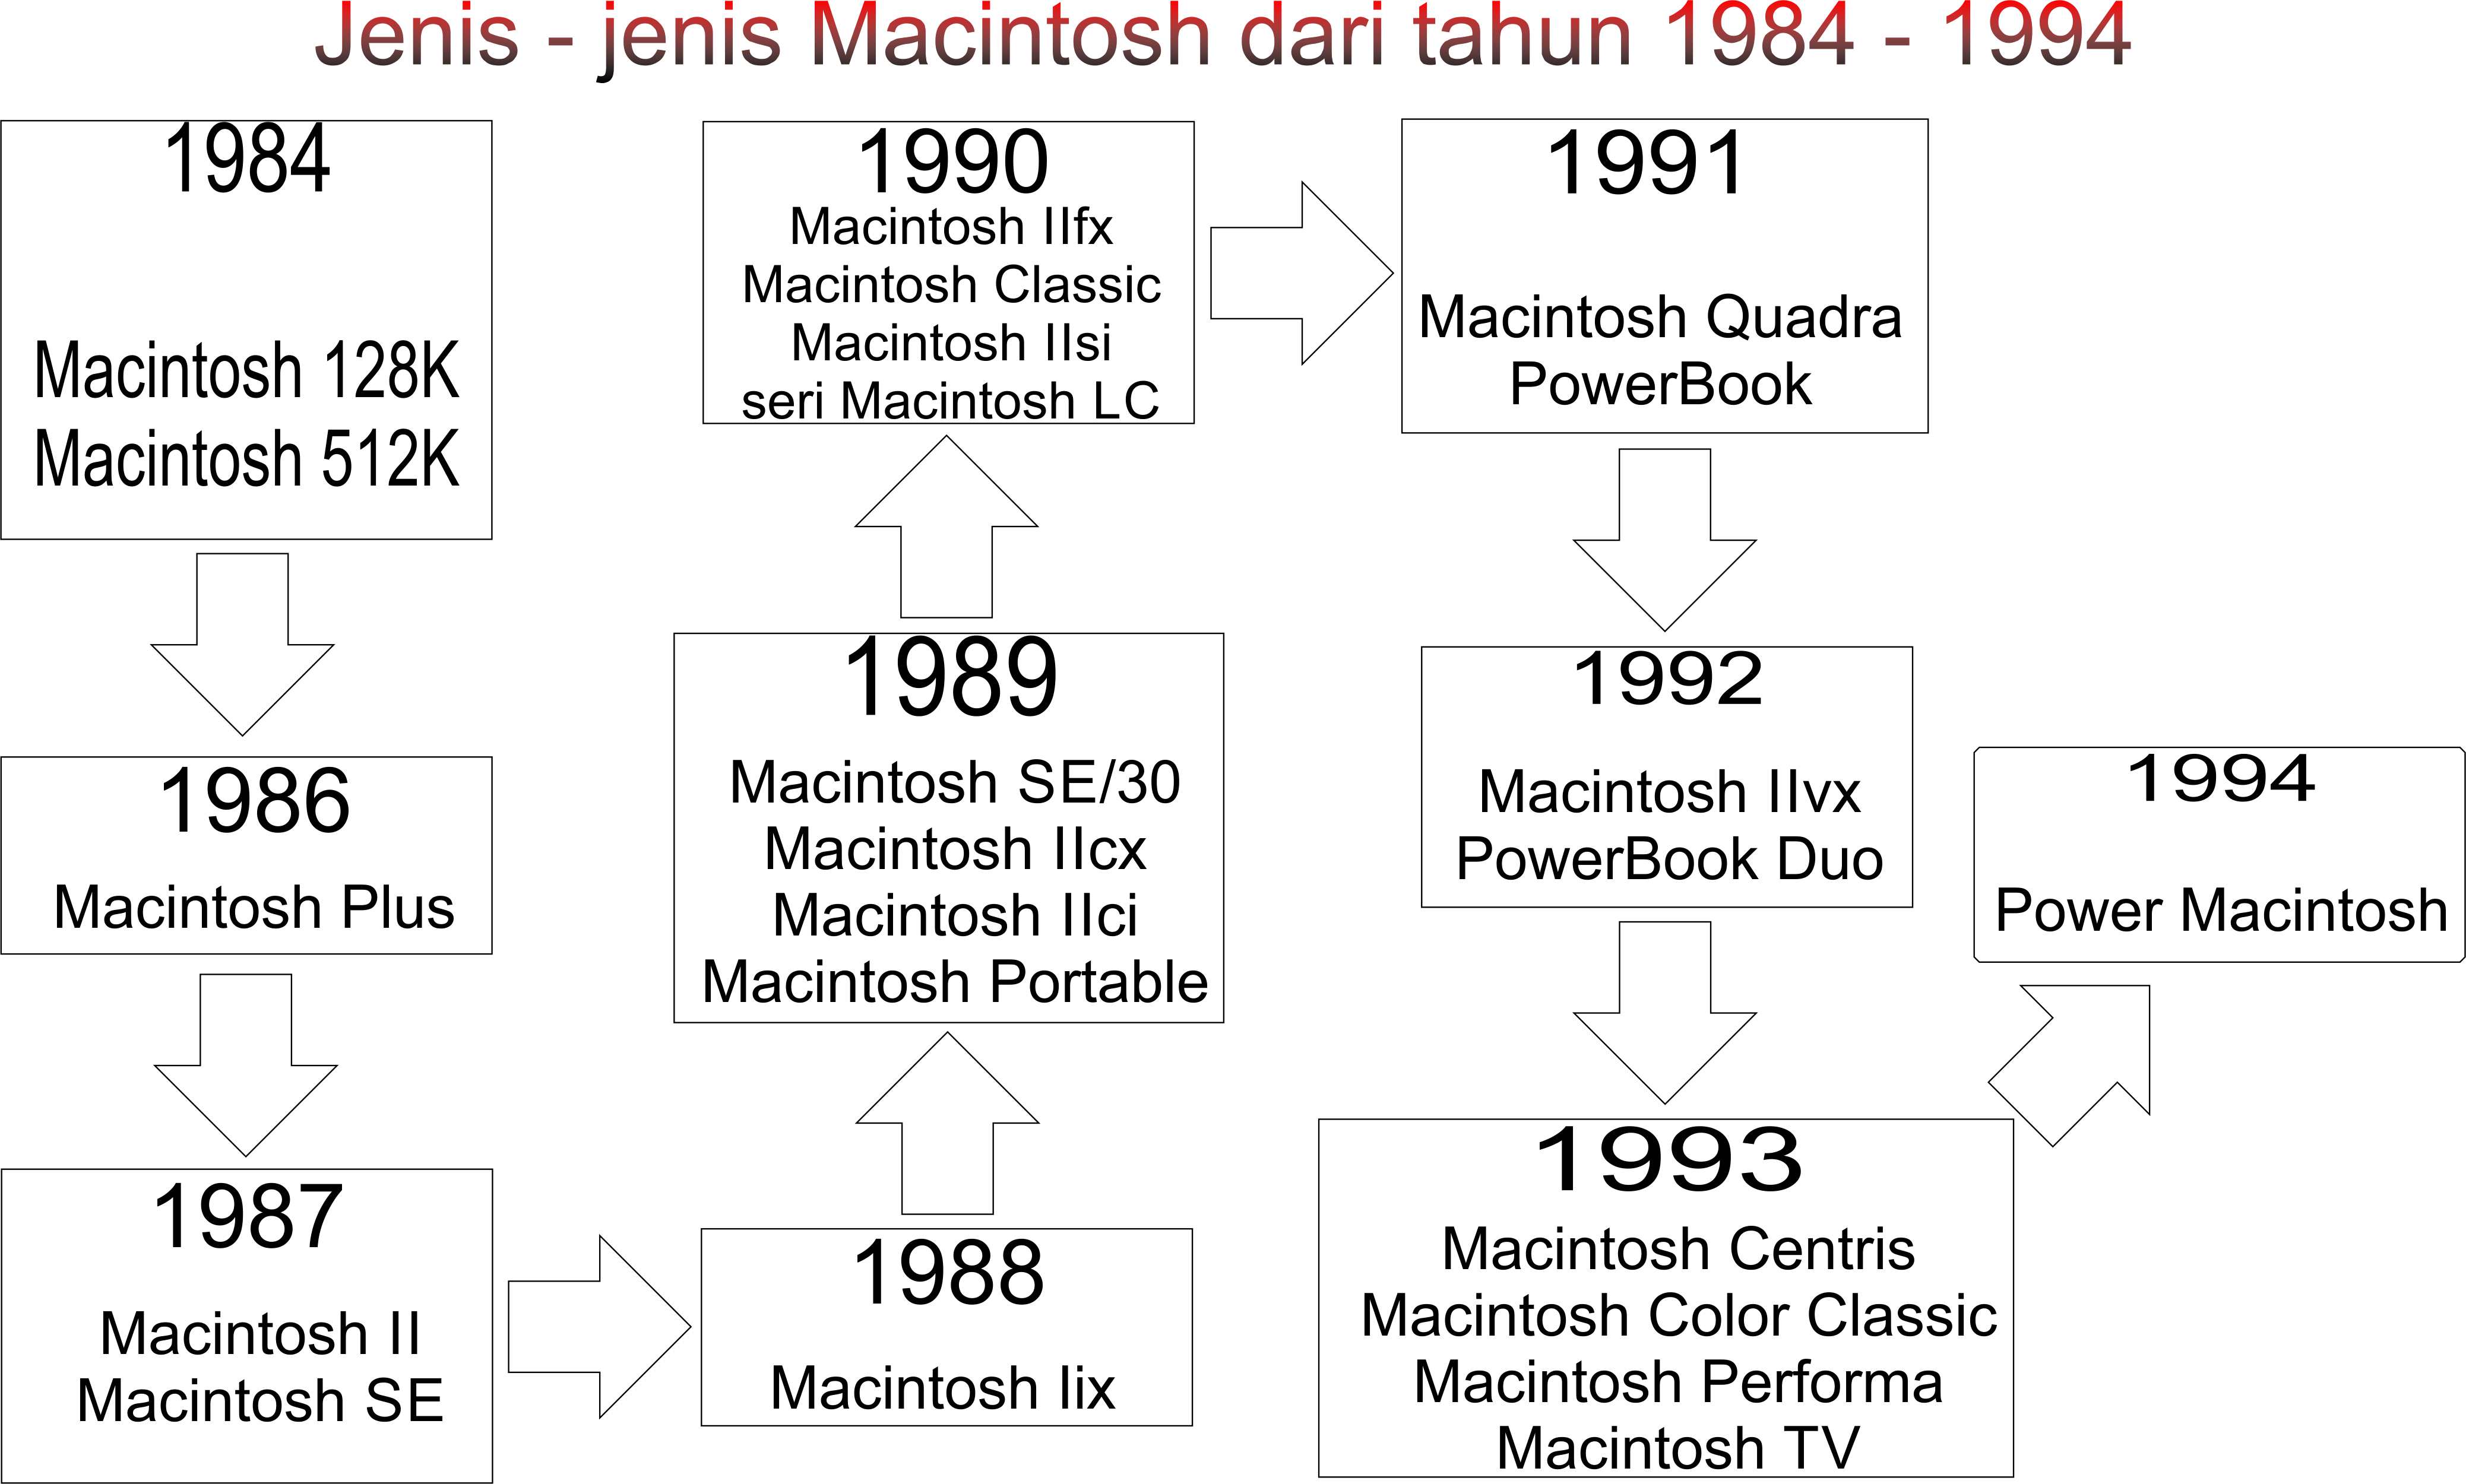
\includegraphics[width=1\textwidth]{figures/Gambar1.JPG}}
	\caption{JenisJenisMacintosh1984-1994.}
	\label{Gambar1}
	\end{figure}

	\ref{Gambar2}
	\begin{figure}[ht]
	\centerline{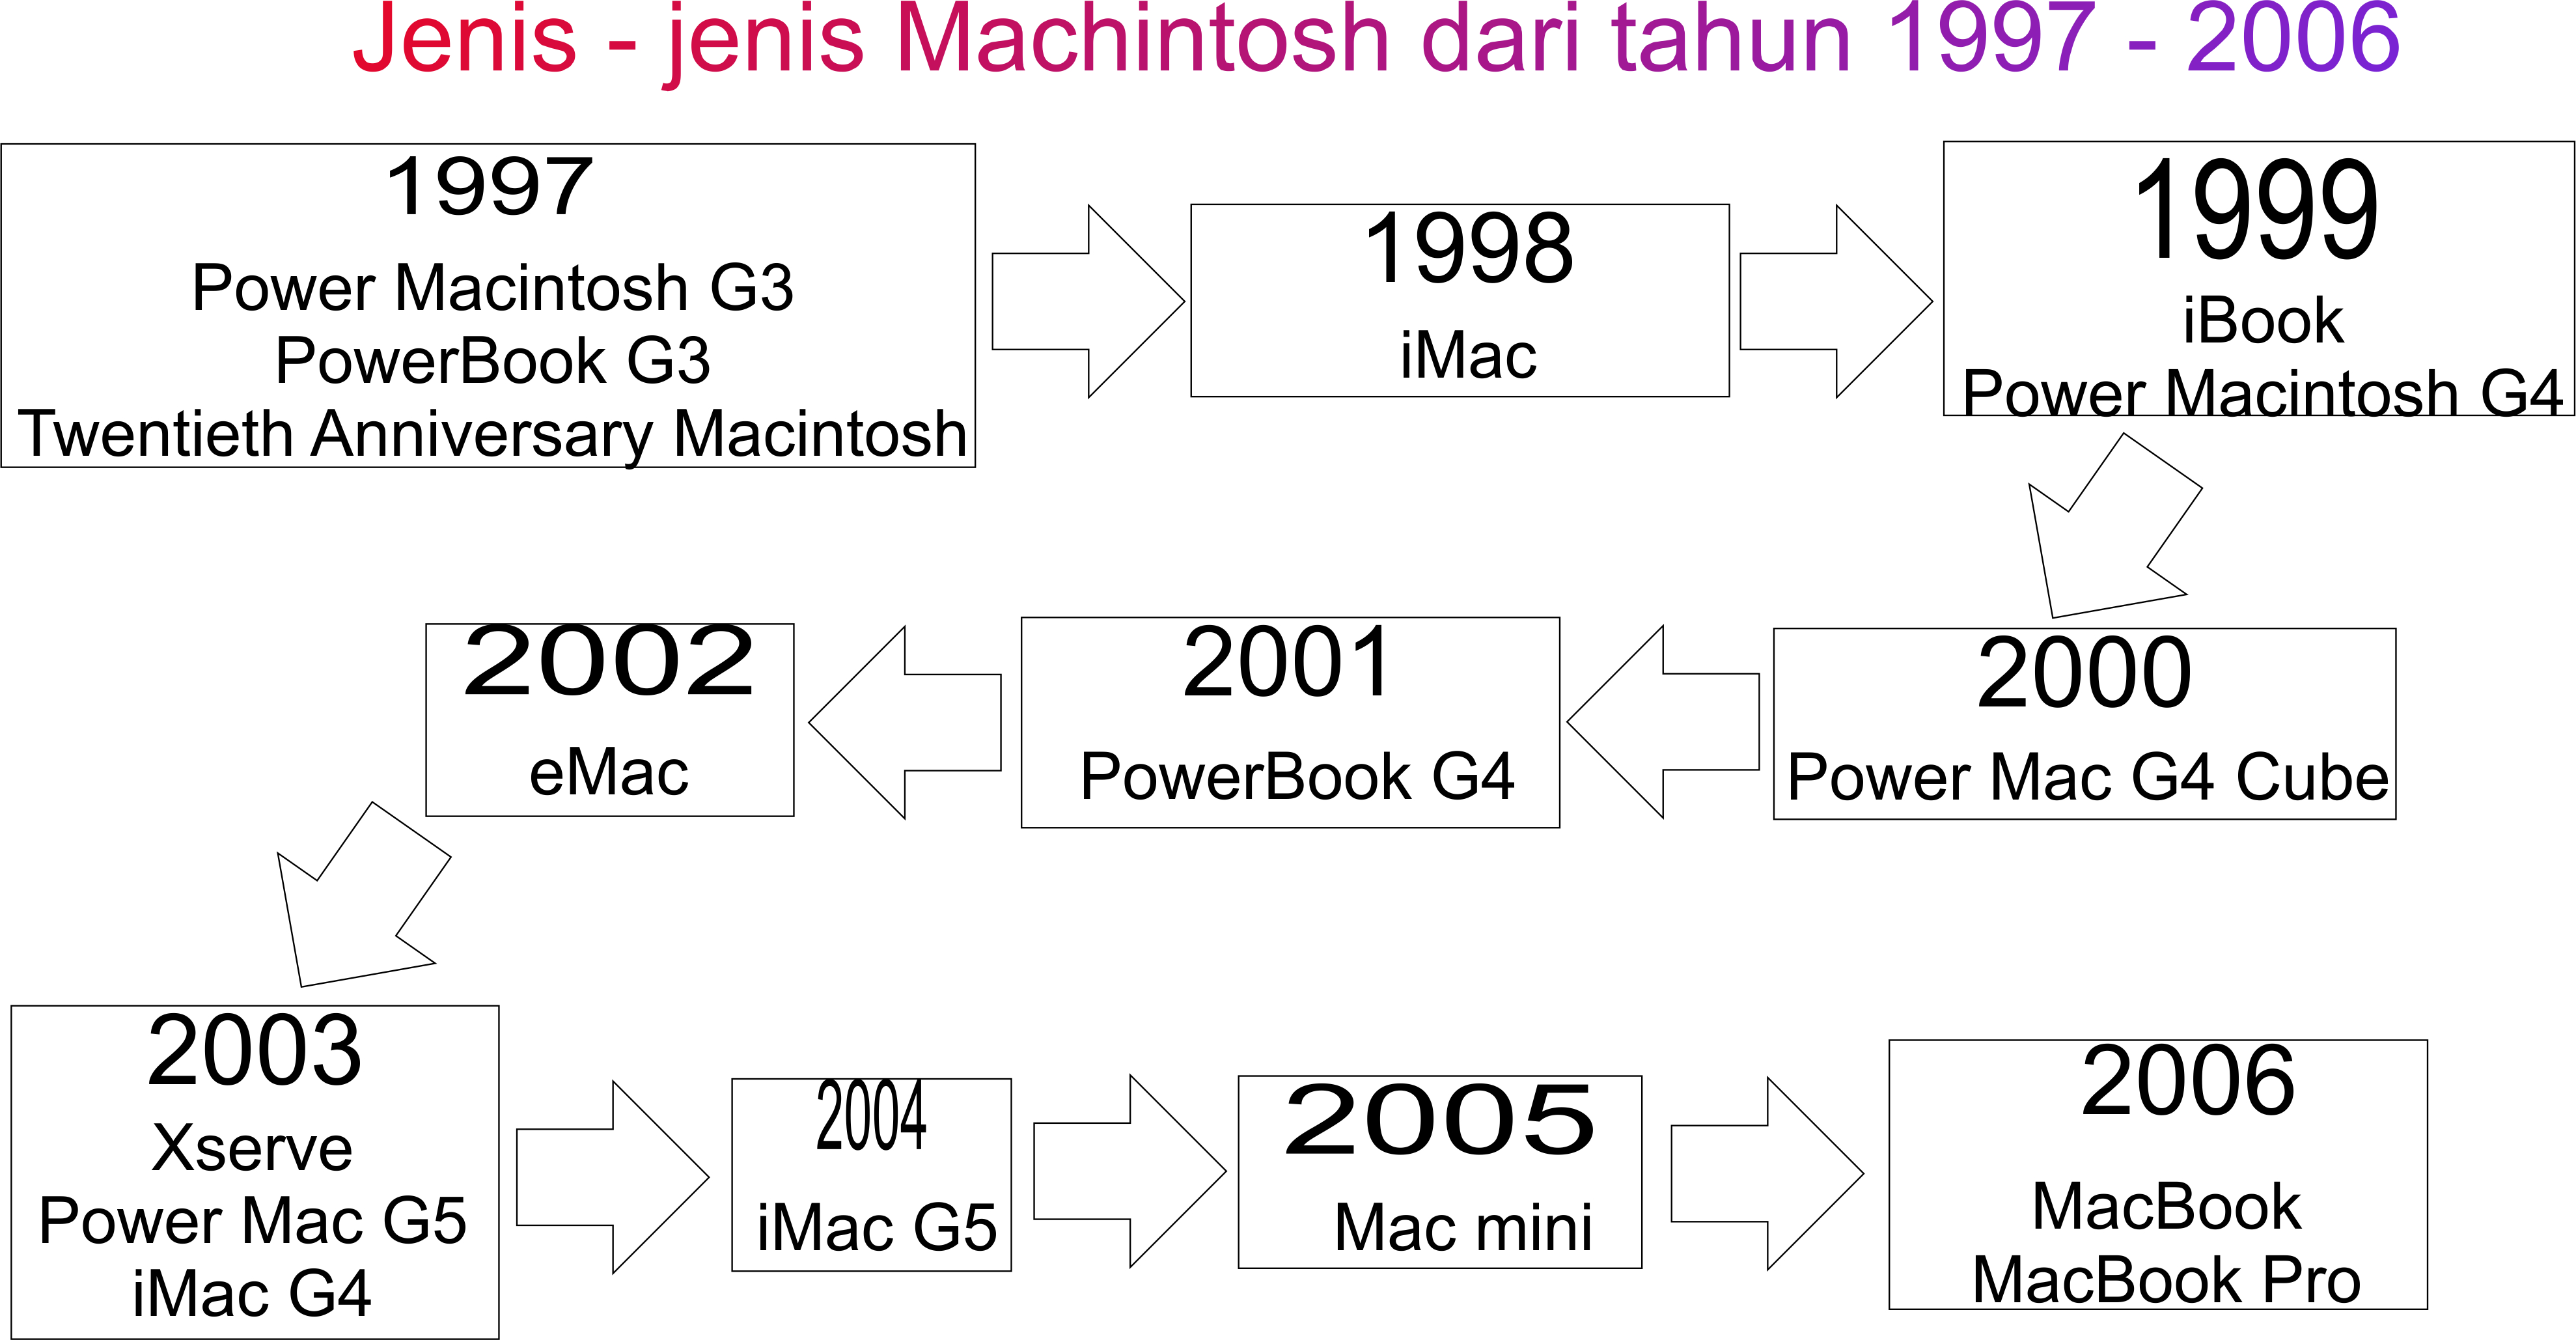
\includegraphics[width=1\textwidth]{figures/Gambar2.JPG}}
	\caption{JenisJenisMacintosh1997-2006.}
	\label{Gambar2}
	\end{figure}

\section{kelebihan dan kekurangan}
Adapun kelebihan dan kekurangan yang dimiliki system operasi Mac OS ini adalah sebagai berikut :

	\subsection{kelebihan}
	-Tampilan yang lebih glossy sehingga bagus untuk desain grafik/multimedia. 
	-Tidak mudah terserang virus, Karena dirancang oleh security oriented. 
	-Machintosh Mempunyai filtur yang bernama “sherlock“ yang fungsinya untuk mencari file pada harddisk dan dalam jaringan lokal, tetapi juga di Internet. 
	-High Performance khususnya untuk MAC OS X yang dapat untuk melakukan semua hal dalam menjalankan aplikasi dengan kecepatan baik. 

	\subsection{kelemahan}
	-Software untuk OS ini belum begitu lengkap seperti pada windows. 
	-Harganya masih terlalu mahal. 
	-Seakan hanya ditujukan untuk desainer grafis. 
	-Kurang cocok untuk aplikasi server dan game. 

Dalam sebuah artikel menyebutkan kekurangan dan kelebihan Mac OS
\cite{linuxwindows}

\section{The Real Leadership Lessons of Steve Jobs}
Enam bulan setelah kematian Jobs, penulis buku biografi terlarisnya mengidentifikasikan praktik yang dapat dicoba oleh setiap CEO.
Steve Jobs mendirikan Apple di garasi orang tuanya pada tahun 1976, digulingkan pada tahun 1985, kembali untuk menyelamatkannya dari kebangkrutan pada tahun 1997, 
dan pada saat dia meninggal, pada bulan Oktober 2011, telah membangun Ini menjadi perusahaan paling berharga di dunia. Sepanjang jalan ia membantu mengubah tujuh industri: 
komputasi personal, film animasi, musik, telepon, komputasi tablet, toko ritel, dan penerbitan digital. Dengan demikian dia termasuk dalam jajaran inovator hebat Amerika, 
bersama Thomas Edison, Henry Ford, dan Walt Disney. Tak satu pun dari orang-orang ini adalah orang suci, tapi lama setelah kepribadian mereka dilupakan, sejarah akan mengingat 
bagaimana mereka menerapkan imajinasi terhadap teknologi dan bisnis. Dalam bulan-bulan sejak biografi Jobs saya keluar, banyak komentator telah mencoba menarik pelajaran manajemen darinya. 
Beberapa dari pembaca itu memiliki wawasan, tapi saya pikir banyak dari mereka (terutama mereka yang tidak memiliki pengalaman kewiraswastaan) tetap mempertahankan sisi kepribadiannya yang kasar. 
Inti dari Jobs, menurut saya, adalah bahwa kepribadiannya adalah bagian integral dari caranya berbisnis. Dia bertindak seolah aturan normal tidak berlaku baginya, dan semangat, intensitas, dan emosionalisme
ekstrim yang ia bawa ke kehidupan sehari-hari adalah hal-hal yang juga dituangkan ke dalam produk yang ia buat. Kelesuan dan ketidaksabarannya merupakan bagian tak terpisahkan dari kesempurnaannya. 
Salah satu terakhir kali saya melihatnya, setelah saya selesai menulis sebagian besar buku ini, saya bertanya lagi tentang kecenderungannya untuk bersikap kasar pada orang lain. \"Lihatlah hasilnya\" 
jawabnya. \"Semua ini adalah orang-orang pintar yang bekerja sama, dan mereka bisa mendapat pekerjaan terbaik di tempat lain jika mereka benar-benar merasa brutal. Tapi mereka tidak melakukannya. 
\"Kemudian dia terdiam beberapa saat dan berkata, dengan sangat sedih\" Dan kami mendapatkan beberapa hal menakjubkan. \"Memang, dia dan Apple memiliki serangkaian hit 
selama belasan tahun terakhir yang lebih besar daripada perusahaan inovatif lainnya di zaman modern: iMac, iPod, iPod nano, Toko iTunes, Toko Apple, MacBook, iPhone, iPad, App Store, 
OS X Lion-tidak untuk
sebutkan setiap film Pixar. Dan saat dia melawan penyakit terakhirnya, Jobs dikelilingi oleh kader rekan yang sangat setia yang telah terinspirasi olehnya selama bertahun-tahun dan istri, 
saudara perempuan, dan empat anak yang sangat mencintai. Jadi saya pikir pelajaran nyata dari Steve Jobs harus diambil dari melihat apa yang sebenarnya dia capai. Saya pernah bertanya 
kepadanya apa pendapatnya tentang ciptaannya yang paling penting, mengira dia akan menjawab iPad atau Macintosh. Sebaliknya dia bilang itu milik Apple perusahaan. Membuat perusahaan 
yang abadi, katanya, jauh lebih sulit dan lebih penting daripada membuat produk hebat. Bagaimana dia melakukannya? Sekolah bisnis akan mempelajari pertanyaan itu satu abad dari sekarang. 
Inilah yang saya anggap kunci suksesnya.
Artikel ini menyebutkan tentang cara kepemimpinan Steve job \cite{isaacson2012real}.

\section{Kesimpulan}
Jadi kesimpulan dari artikel mengenai Macintosh atau MacOS yang telah dapat kita rasakan dari awal kemunculannya pada tahun 1984 hingga saat ini pada tahun 2017 MacOS memiliki 2 jenis yaitu Jenis Mac OS Classic (Klasik) dan Mac OS X sudah Berkembang menjadi banyak Series seperti yg pertama di keluarkannya yaiu System 1, System 2,3,\& 4 hingga yg terakhir dalam MacOS Klasik yaitu MacOS 9 pada tahun 1999. Dan juga dari Mac OS X yang hingga kini dapat kita peroleh dan rasakan mulai dari MacOS X 10.0 dengan nama lain yaitu \"Cheetah\" pada tahun 2001 hingga yang paling terbaru yaitu versi terbaru atau revisian dari Mac OS versi 10.12 yaitu Sierra dengan nama dan serial baru yaitu \"High Sierra\" dengan nomor seri 10.13 yang baru saja rilis pada 2017 ini

%\chapter[Free BSD]
%{Software\\ bsd}
%% Nama Kelompok : FreeBSD
% Kelas         : D4 Teknik Informatika 1A
% Anggota       :
% 1. Jeremia Wahyudi Sianturi		1174029
% 2. Dwiyulianingsih				1174009
% 3. Arjun Yuda Firwanda			1174008
% 4. Dwi Septiani Tsaniyah			1174003
% 5. Ervanda Rambu Anarky			1174007
% 6. Muh. Rifky	Prananda			1174017
\section{FreeBSD}
	FreeBSD adalah suatu sistem operasi bersifat open source bertipe UNIX bebas yang diturunkan dari UNIX AT\&T lewat cabang Berkeley Software distribution
	BSD. FreeBSD adalah salah satu keluarga BSD yang saat ini banyak digunakan dan dikembangkan pada berbagai kalangan individu,
	perusahaan, dan bahkan universitas. Bila dibandingkan dengan windows FreeBSD relatif lebih sulit dalam penggunaannya, karenya masih bersifat text base
	dalam memberikan command sedangkan windows memiliki GUI yang jauh lebih dibandingkan FreeBSD keunggulan FreeBSD dibanding windows
	adalah kebebasan dalam penggunaannya bahkan pengembangan dari sistem operasi tersebut lisensinya sudah dijamin untuk kebebasan.
	FreeBSD mengoptimalkan penggunaan flatform PC. FreeBSD menyediakan kemudahan dalam penggunaan instalasi dan dukungan yang luas terhadap perangkat keras dalam PC.
	FreeBSD mendukung arsitektur i386 dan Alpha, dan pengembangannya pada beberapa flatform telah dilakukan.
	\ref{index} 
	\begin{figure} [ht]
	\centerline{
\includegraphics[width=1\textwidth]{figures/index.jpg}}
	\caption{gambarindex}
	\label {index}
	\end {figure}
\subsection{Sejarah}
	menurut \cite{luanmembangun} menyebutkan bahwa :
	Berkeley software distribution diawali dari modifikasi AT\&T Unix software, sebelum berkembang menjadi suatu proyek yang signifikan. Namun sayangnya, AT\&T masih memegang lisensi untuk UNIX dan bertentangan dengan Berkeley Software Design Inc. BSDI yang mengklaim bahwa Berkeley Software Distribution juga termasuk source code AT\&T.
	Kasus lisensi ini sempat dibawa ke pengadilan, dan diproses yang kemudian  menghasilkan bahwa Bill Jolitz berwenang untuk mengambil bagian dari software yang bukan berasal dari AT\&T dan kemudian mengembalikannya menjadi free UNIX. Ini merupakan sebuah awal baru dari lahirnya modern BSD.
	Dalam pengembangannya FreeBSD melibatkan begitu banyak pihak yang notabene merupakan programmer individu berkemampuan tinggi yang dikenal sebagai commiters. Commiters ini dipilih oleh FreeBSD core team dan memiliki wewenang langsung untuk melakukan suatu perubahan-perubahan pada system yang  berjalan.
	FreeBSD lahir pada tahun 1992 saat Jordan K. Hubbard, Rob Grimes, dan Nate Williams merilis sebuah paket yang dikenal dengan unofficial 386BSD patchkit. Dari sana lahirlah suatu mekanisme yang membentuk 386BSD 0.5 1/2, akan tetapi pada 1993 Jolitz mencabut persetujuan pada proyek tersebut dan melahirkan FreeBSD. 
	Jordan K Hubbard dan David Greenman kemudian membentuk suatu kerjasama untuk mempersiapkan sebuah proyek CDROM FreeBSD versi 1.0 berbasis Net/2 yang telah dirilis pada bulan desember tahun 1993, setelah itu pada bulan November 1994 versi kedua dari FreeBSD dirilis yaitu versi 2.0 yag tidak lagi 
	berbasis Net/2 tetapi telah diupgrade menjadi berbasis 4.4BSD BSD dibuat, dikembangkan serta digunakan secara bebas sebagai perlawanan terhadap lisensi UNIX yang dimiliki oleh AT\&T. oleh karena itu BSD mempunyai lisensi sendiri yang memungkinkan setiap individu bebas melakukan pengembangan dan
	FreeBSD telah digunakan diseluruh penjuru internet oleh beberapa perusahaan yang memiliki orientasi pada internet. sebagai contohnya saat ini the \"babybell\" US west menggunakan FreeBSD untuk menjalankan operasional internet. IBM, Nokia, dan banyak perusahaan hardware menggunakan FreeBSD pada embedded system.
	dalam kenyataannya jika sebuah perusahaan serius untuk melakukan manajemen bandwich internet, kemungkinan besar sistemnya menjalankan FreeBSD.
	saat ini FreeBSD memiliki hampir 300 developer. comitters mempunyai hak read-and-write atas master source code dan dapat men-develop, debug, atau memperbaiki kulaitas bagian yang dianggap penting.
	sebagai contoh, developmen networking dibahas dalam milis-milis yang banyak tersebar di media sosial ada pula beberapa chanel IRC untuk mendiskusikan banyak hal mengenai FreeBSD.
	para committers bertanggung jawab agar FreeBSD tetap berjalan dan memabah fitur baru serta mengevaluasi patch yang dikirim oleh para kontributor. 
	hingga akhirnya FreeBSD memiliki users yang jauh lebih banyak karena kita dapat mendownload keseluruhan FreeBSD dengan gratis dan tidak perlu register, upgrade atau mengirim email ke mailing list.

\subsection{VarianFreeBSD}
	Varian dari FreeBSD kami mendapatkan referensi dari \cite{nugroho2015analisis} yang kami kembangkan menjadi :
	FreeBSD memiliki dua versi saat dirilis. versi tersebut antara lain versi-CURRENT dan versi-STABLE. selain itu varian FreeBSD juga ada UNIX FreeBSD, NETBSD, OpenBSD, UNIX lainnya, dan AIX yang dikenal dapat dijalankan pada banyak jenis arsitektur, dan FreeBSD yang mendukung flatform X86, AMD64, IA64, SPARC64, dan Alpha.
	FreeBSD 6.0 dikenal dengan stabilitas, performa, dan keamannanya sehingga digunakan oleh banyak perusahaan di seluruh dunia. rilis UNIX freeBSD yang digunakan saat ini adalah versi 6.2. 
	Sebenarnya masih banyak lagi jenis-jenis sistem operasi yang dapat dikatakan berbasis dengan FreeBSD seperti IRIX, HPUX, LINUX, Sun Solaris, Mac OS X, BSD/OS dan juga masih ada lagi yang belum disebutkan tapi mungkin karena berikut merupakan kesimpulan sederhana jadi tidak dijelaskan secara semua atau dapat dikatakan menyeluruh. 
	Jadi dapat ditarik bahwa banyak jenis-jenis dari OS FreeBSD yang telah disebutkan.
	pengembangan gentoo/FreeBSD menggunakan versi ini, sedangkan  pengembangan dengan versi lama telah dihentikan dan tidak lagi didukung. pada varian BSD NETBSD dan OPENBSD memiliki modal pengembangan sistem operasi yang terbuka akan tetapi memiliki susanan tertentu yaitu :
	1. contributor, adalah developer yang menulis kode, patch atau dokumentasi, akan tetapi tidak memiliki hak untuk menulis atau membuat suatu file dalam source tree. jika pekerjaan yang mereka lakukan ingin dimasukkan maka harus diperiksa terlebih dahulu oleh committers atau dengan persetujuan beberapa orang committers
	2. commiters adalah developer yang memiliki hak menulis dan mengakses source tree, dalam lingkup cvs, memiliki hak commit secara tipikal dan hanya bekerja dalam bagian terpilih di suatu proyek.
	3. coreteam memiliki wewenang untuk membimbing secara keseluruhan arah dan tujuan proyek, dan membuat keputusan akhir dalam kasus berselisih paham antar developer mengenai source code atau hal-hal lain. OpenBSD tidak memiliki coreteam secara formal namun Theo De Raadt bertugas sebagai pemimpin proyek.
	setap orang dapat menjadi contributor dengan mengirimkan patch atau membenarkan kesalahan penulisan dalam sebuah halaman manual orang yang mengkontribusikan banyak hal, atau berkompeten dalam suatu proyek akan dipeomosikan menjadi commiters yang ditujukan untuk menjaga committers yang lain memeriksa terlalu banyak hal dalam waktu yang sama.
\subsubsection{versi-CURRENT}
	versi-CURRENT merupakan versi yang pertama kali dirilis biasanya versi ini dipakai oleh para develover yang sudah mahir mengenai
	cara kerja dari FreeBSD agar dapat menemukan berbagai bugs paska produksi. setelah versi-CURRENT diperbaiki maka versi tersebut
	akan menjadi versi stable yang siap digunakan karena dalam versi-CURRENT kurang familiar bagi pengguna baru FreeBSD.
	\ref{freebsd} 
	\begin{figure} [ht]
	\centerline{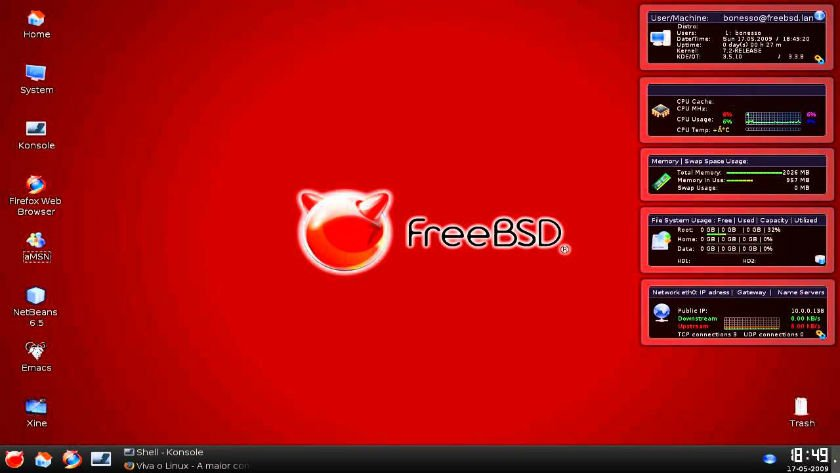
\includegraphics[width=1\textwidth]{figures/freebsd.jpg}}
	\caption{gambarindex}
	\label {freebsd}
	\end {figure}
\subsection{Sejarah}
\subsubsection{versi-STABLE}
	versi-STABLE adalah versi pengembangan ddari versi sebelumnya yaitu versi-CURRENT yang dianggap kurang familiar.
	versi-STABLE siap digunakan oleh siapapun yang baru mencoba FreeBSD karena versi sebelumnya hanya ditujukan kepada
	orang yang mahir dalam mengidentivikasi masalaah yang muncul pada versi tersebut.
\subsubsection{NETBSD}
	NetBSD dapat juga dikatakan mirip dengan FreeBSD dalam berbagai macam bentuk dan aspek. Kedua proyek ini saling berbagi source code dan developer. 
	Tujuan paling utama dari NetBSD adalah membuat sistem operasi yang dapat diporting ke berbagai macam plattform hardware. 
	Sebagai contohnya bahwa NetBSD dapat berjalan di berbagai macam plattform hardware yaitu : bahwa NetBSD dapat berjalan di VAXes, PocketPC, Alpha server, dan Compaq iPaq. Bahkan NetBSD dapat berjalan juga pada hardware yang belum ada (belum diluncurkan). 
	Source code NetBSD diberikan secara bebas, sama seperti pendahulunya, FreeBSD.
\subsubsection{openBSD}
	OpenBSD merupakan cabang dari NetBSD mulai tahun  1996, tujuan utam dari OpenBSD adalah membuat OS BSD yang aman. 
	OpenBSD adalah BSD yang pertama kali men-suport hardware-accelerated crytography {membolehkan untuk men-encrypt dan decrypt informasi pada waktu yang singkat, para developenya sangat bangga karena faktanya, default instalasi OpenBSD tidak dapat di-hack selama kira-kira 4 tahun.
\subsubsection{UNIXFreeBSD}
	FreeBSD dapat dikatakan mirip dengan sistem operasi Unix yang bebas {berlisensi}. Pada tahun 1993 ketika pengembangan 386BSD dihentikan, maka lahirlah dua proyek baru yang satu dikenal dengan nama Net BSD, yang dikenal dapat dijalankan pada banyak jenis arsitektur, 
	dan yang satunya lagi dikenal dengan sebutan FreeBSD yang mendukung platform x86, amd64, ia64, sparc64 dan alpha. 
	Free BSD 6.0 dikenal juga denagn stabilitas, performa dan keamanannya sehingga sering digunakan oleh perusahaan-perusahaan terkenal yang ada di seluruh dunia. 
	Saat ini unix FreeBSD yang digunakan adalah versi 6.2. Dan sebentar lagi juga akan keluar pengembangan  Gentoo/FreeBSD versi terbaru, sedangkan versi lama yang ingin dikembangkan malah diberhentikan proyeknya dan tidak didukung sama sekali pembentukannya. 
	Pasti kita semua bertanya-tanya apa itu Gentoo/FreeBSD? Baiklah akan dijelaskan bahwa Gentoo/FreeBSD adalah subproyek dari proyek Gentoo/Alt, Yang tujuannya hanya untuk menyediakan sistem operasi FreeBSD berkemampuan penuh dengan mengambil rancangan dari Gentoo Linux, seperti sistem unit dan sistem manajemen paket Portage.
\subsubsection{UNIXLainnya}
	Masih ada beberapa UNIX OS di luar sana, beberapa bahkan menyewa nama trademark dari UNIX sehingga mereka dapat menyebut diri mereka itu UNIX
\subsubsection{AIX}
	Salah satu pesaing ketat dari UNIX adalah IBM AIX. AIX mengklaim bahwa mereka mempunyai journaling filesystem terbaik seperti, mampu mencatat seluruh disk transaction yang terjadi, sehingga mereka mampu me-recover system tanpa banyak masalah kemampuan ini meningkatkan reliability. 
	Dan AIX juga berbasis BSD.
\subsection{Tujuan}
	Tujuan dari adanya software ini adalah untuk menyediakan software yang tentu saja dapat digunakan dalam berbagai kepentingan dengan mudah dan gratis (free). karena software ini disediakan dengan gratis dan dapat digunakan oleh siapa saja termasuk untuk meraih kepentingan komersil, 
	source kode yang tersedia dengan gratis siapun dapat meningkatkan  peforma melalui free bsd ini atau memungkinkan bug mensubmit source codenya dan dapat digunakan sesuai dengan keinginan si pengguna.
	Tujuan dari adanya versi-CURRENT dan versi-STABLE adalah untuk memberitahukan fixed bugs bagi para pengguna
	dan meyakinkan pengguna dengan fitur - fitur terbaru dan masalah yang telah diatasi. selain perbedaan diantara versi-CURRENT dan versi-STABLE
	pemberian nama dari versi-STABLE juga telah dibuat sedemikian rupa hingga para penggguna tahu  perbaikan - perbaikan yang telah dilakukan.
\subsection{kegunaanFreeBSD}
	pada saat ini FreeBSD dikenal sebagai network administrator operating system karena FreeBSDberjalan dengan cepat dan telah banyak tersedia berbagai networking tools. selain itu, FreeBSDdapat berjalan denngan cepat dan efisien didalam sebuah laptop untuk menjalankan aplikasi perkantoran, atau sebagai email client maupun email database.
	instalasi dari FreeBSD dapat dikatakan cukup mudah bagi yang sudah pernah menginstall system operasi windows.
\subsection{keuntungandankelemahan}
	keuntungan dan kelemahan kami mengambil referensi dari : \cite{nugroho2015analisis}
	keuntungan :
	1. FreeBSDdapat berjalan lebih cepat daripada LINUX dalam beberapa bagian misalnya sebagai server NFS
	2. dalam aplikasi server secara prinsip BSD sama baiknya dengan LINUX
	kelemahan :
	1. FreeBSD tidak dapat digunakan pada microkanal lama
	2. FreeBSD tidak dapat mendukung ISA-plug-and-play-card
	3. FreeBSD tidak bisa menandingi perkembangan LINUX yang cepat karena kurangnya developer
	4. FreeBSD belum jelas masa depannya untuk server database
\subsection{Kesimpulan}
	Dari penjelasan diatas dapat disimpulkan bahwa FREEBSD mempunyai banyak fitur-fituryang dapat dipelajari satu per satu. Dan ada kelebihan, kekurangan yang ada di FREEBSD, diataranya banyaknya tersedia aplikasi dan program file gratis. 
	Mudah di kustomisasi atau dapat dirubah-rubah secara bebas. Freebsd mempunyai fitur multiuser, bersifat opensource, memiliki sistem software third-party yang memberikan kemudahan yang berarti bagi para user untuk menambah atau menghapus aplikasi-aplikasi.
	Para user cukup mengeksekusi satu baris perintah dan aplikasi-aplikasi dengan sendirinya di download dan diinstal secara otomatis, sehingga tugas-tugas didalam system Freebsd menjadi mudah dan praktis. 
	Dari beberapa kelebihan diatas secara progaming Freebsd dapat dikatakan system yang dapat mempermudah user dalam menggunakan dalam berbagai tugas-tugas system operasi.
	Di dalam Freebsd terdapat kekurangan juga, diantaranya relatif penggunaannya sulit karena masih dalam bentuk text base dalam mengcommandnya, artinya dalam memerintahnya masih sulit. Tidak mendukung ISA plug and play chard, artinya tidak dapat memasang dan memainkan. 
	Kecilnya basis developer dan pemakai yang mencari bug/kelemahan program.
	Operating sistem ini dinamakan freeBSD karena software ini gratis untuk digunakan oleh siapapun termasuk untuk kepentingan komersial, source code yang tersedia dengan gratis, siapapun dapat meningkatkan performa freeBSD ini atau menemukan bug
	(Pengertian bug adalah kesalahan pada komputer baik disebabkan oleh perangkat lunak ataupun perangkat keras sehingga komputer tidak bekerja dengan semestinya ) untuk mensubmit souce codenya, kata ‘free’ dapat diartikan sebagai gratis, atau dapat digunakan sesuai keinginan user.
	FreeBSD dikenal sebagai network administrator operating system karena FreeBSD berjalan dengan cepat dan telah banyak tersedia berbagai networking tools. 
	selain itu, FreeBSD dapat berjalan denngan cepat dan efisien didalam sebuah laptop untuk menjalankan aplikasi perkantoran, atau sebagai email client maupun email database.
	FreeBSD dapat dikatakan cukup mudah bagi yang sudah pernah menginstall system operasi windows.
	FreeBSD dapat berjalan di personal komputer yang menggunakan sistem arsitektur Intel. Artinya dapat mendapatkan secara gratis tanpa berbayar.


%\chapter[Android]
%{Software\\ android}
%\input{chapter/android.tex}


%%%%%%%%%%%%%%%%%%%%%%%%%%%%%%%%%%%%%%%%%%%%%%%%%%%%%%
%% optional prologue or prologues
% \chapter{Chapter Title}
% \prologue{<text>}{<author attribution>}

%%%%%%%%%%%%%%%%%%%%%%%%%%%%%%%%%%%%%%%%%%%%%
% Edited Book: Author and Affiliation
%%%%%%%%%%%%%%%%%%%%%%%%%%%%%%%%%%%%%%%%%%%%%

% After \chapter{Chapter Title}, you can
% enter the author name and embed the affiliation with
% \chapterauthors{(author name, or names)
% \chapteraffil{(affiliation or affiliations)}
% }    

% For instance:
% \chapter{Chapter Title}
% \chapterauthors{G. Alvarez and R. K. Watts
% \chapteraffil{Carnegie Mellon University, Pittsburgh, Pennsylvania}

% For separate affiliations you can use \affilmark{(number)} after
% the name of a particular author and before the matching affiliation:

% For instance:
% \chapter{Chapter Title}
% \chapterauthors{George Smeal, Ph.D.\affilmark{1}, Sally Smith,
% M.D.\affilmark{2}, and Stanley Kubrick\affilmark{1}
% \chapteraffil{\affilmark{1}AT\&T Bell Laboratories
% Murray Hill, New Jersey\\
% \affilmark{2}Harvard Medical School,
% Boston, Massachusetts}
% }

%%%%%%%%%%%%%%%%%%%%%%%

%% short version of section head, or one without \\ supplied in sq. brackets.

% \section[Introduction and fugue]{Introduction\\ and fugue}
% \subsection[This is the subsection]{This is the\\ subsection}
% \subsubsection{This is the subsubsection}
% \paragraph{This is the paragraph}

% \begin{chapreferences}{widest label}
% \bibitem{<label>}Reference
% \end{chapreferences}

% optional chapter bibliography using BibTeX,
% must also have \usepackage{chapterbib} before \begin{document}
% Must use root file with \include{chap1}, \include{chap2} form.
%\bibliographystyle{plain}
%\bibliography{<your .bib file name>}

% optional appendix at the end of a chapter:
% \chapappendix{<chap appendix title>}
% \chapappendix{} % no title

%%%%%%%%%%%%%%%%%%%%%%%%%%%%%%%%%%%%%%%%%%%%%%%%%%%%%%%%%%%%%%%%
%% End Matter >>>>>>>>>>>>>>>>>>

% \appendix{<optional title for appendix at end of book>}
% \appendix{} % appendix without title

% \begin{references}{<widest label>}
% \bibitem{sampref}Here is reference.
% \end{references}

%%%%%%%%%%%%%%%%%%%%%%%%%%%%%%%%%%%%%%%%%%%%%%%%%%%%%%%%%%%%%%%%
%% Optional Problem Sets: Can use this at the end of each chapter or at end
%% of book

% \begin{problems}
% \prob
% text

% \prob
% text

% \subprob
% text

% \subprob
% text

% \prob
% text
% \end{problems}

%%%%%%%%%%%%%%%%%%%%%%%%%%%%%%%%%%%%%%%%%%%%%%%%%%%%%%%%%%%%%%%%
%% Optional Exercises: Can use this at the end of each chapter or at end
%% of book

% \begin{exercises}
% \exer
% text

% \exer
% text

% \subexer
% text

% \subexer
% text

% \exer
% text
% \end{exercises}


\bibliographystyle{IEEEtran}
\bibliography{IEEEabrv,windows,linux,mac,android}

%%%%%%%%%%%%%%%%%%%%%%%%%%%%%%%%%%%%%%%%%%%%%%%%%%%%%%%%%%%%%%%%
%% INDEX: Use only one index command set:

%% 1) The default LaTeX Index
\printindex

%% 2) For Topic index and Author index:

% \usepackage{multind}
% \makeindex{topic}
% \makeindex{authors}
% \begin{document}
% ...
% add index terms to your book, ie,
% \index{topic}{A term to go to the topic index}
% \index{authors}{Put this author in the author index}

%% (these are Wiley commands)
%\multiprintindex{topic}{Topic index}
%\multiprintindex{authors}{Author index}

\end{document}

%%%%%%% Demo of section head containing sample macro:
%% To get a macro to expand correctly in a section head, with upper and
%% lower case math, put the definition and set the box 
%% before \begin{document}, so that when it appears in the 
%% table of contents it will also work:

\newcommand{\VT}[1]{\ensuremath{{V_{T#1}}}}

%% use a box to expand the macro before we put it into the section head:

\newbox\sectsavebox
\setbox\sectsavebox=\hbox{\boldmath\VT{xyz}}

%%%%%%%%%%%%%%%%% End Demo


Other commands, and notes on usage:

-----
Possible section head levels:
\section{Introduction}
\subsection{This is subsection}
\subsubsection{This is subsubsection}
\paragraph{This is the paragraph}

-----
Tables:
 Remember to use \centering for a small table and to start the table
 with \hline, use \hline underneath the column headers and at the end of 
 the table, i.e.,

\begin{table}[h]
\caption{Small Table}
\centering
\begin{tabular}{ccc}
\hline
one&two&three\\
\hline
C&D&E\\
\hline
\end{tabular}
\end{table}

For a table that expands to the width of the page, write

\begin{table}
\begin{tabular*}{\textwidth}{@{\extracolsep{\fill}}lcc}
\hline
....
\end{tabular*}
%% Sample table notes:
\begin{tablenotes}
$^a$Refs.~19 and 20.

$^b\kappa, \lambda>1$.
\end{tablenotes}
\end{table}

-----
Algorithm.
Maintains same fonts as text (as opposed to verbatim which uses fixed
width fonts). Space at beginning of line will be maintained if you
use \ at beginning of line.

\begin{algorithm}
{\bf state\_transition algorithm} $\{$
\        for each neuron $j\in\{0,1,\ldots,M-1\}$
\        $\{$   
\            calculate the weighted sum $S_j$ using Eq. (6);
\            if ($S_j>t_j$)
\                    $\{$turn ON neuron; $Y_1=+1\}$   
\            else if ($S_j<t_j$)
\                    $\{$turn OFF neuron; $Y_1=-1\}$   
\            else
\                    $\{$no change in neuron state; $y_j$ remains %
unchanged;$\}$ .
\        $\}$   
$\}$   
\end{algorithm}

-----
Sample quote:
\begin{quote}
quotation...
\end{quote}

-----
Listing samples

\begin{enumerate}
\item
This is the first item in the numbered list.

\item
This is the second item in the numbered list.
\end{enumerate}

\begin{itemize}
\item
This is the first item in the itemized list.

\item
This is the first item in the itemized list.
This is the first item in the itemized list.
This is the first item in the itemized list.
\end{itemize}

\begin{itemize}
\item[]
This is the first item in the itemized list.

\item[]
This is the first item in the itemized list.
This is the first item in the itemized list.
This is the first item in the itemized list.
\end{itemize}

%% Index commands
Author and Topic Indices, See docs.pdf and w-bksamp.pdf
